\documentclass[a4paper,twoside,11pt]{book}
%\documentclass[a4paper,twoside,11pt,titlepage]{book}
\usepackage{listings}
\usepackage[utf8]{inputenc}
\usepackage[spanish,es-tabla]{babel}
%%\usepackage{import} no lo encuentra, sirve para algo?
\usepackage[pdftex]{graphicx}
\usepackage{titlesec}
\usepackage{wrapfig}
\usepackage{url}
\usepackage{index}
\usepackage{enumitem}
\usepackage{caption}
\usepackage{booktabs} % Para formatos especiales de tablas
\usepackage{float}    % Posicionamiento avanzado de gráficos
\usepackage{subcaption} % Captions con figuras enlazadas
\usepackage{adjustbox}
\usepackage{amsmath}
\usepackage{amsfonts}
\usepackage{mathtools}

% Lista de acrónimos
\usepackage[acronym,shortcuts]{glossaries}
\makeglossaries
%
% Lista de acrónimos
% 
% Autor: Felipe Torres González
% Temática: WR-es
%
\newacronym{gnss}{GNSS}{Global Navigation Satellite System}
\newacronym{wr}{WR}{White-Rabbit}
\newacronym{ptp}{PTP}{Precision Time Protocol}
\newacronym{synce}{Sync-E}{Synchronous Ethernet}
\newacronym{ns}{ns}{nanosegundos}
\newacronym{hm}{H-maser}{Hydrogen maser}
\newacronym{ntp}{NTP}{Network Time Protocol}
\newacronym{gpsdo}{GPSDO}{GPS disciplined oscillator}
\newacronym{gps}{GPS}{Global Positioning System}
\newacronym{pps}{PPS}{Pulse Per Second}
\newacronym{lan}{LAN}{Local Area Network}
\newacronym{ieee}{IEEE}{Institute of Electrical and Electronics Engineers}
\newacronym{oc}{OC}{Ordinary Clock}
\newacronym{bc}{BC}{Boundary Clock}
\newacronym{gm}{GM}{GrandMaster}
\newacronym{tc}{TC}{Transparent Clock}
\newacronym{osi}{OSI}{Open System Interconnection}
\newacronym{bmc}{BMC}{Best Master Clock}
\newacronym{cern}{CERN}{Organización Europea para la Investigación Nuclear}
\newacronym{spec}{SPEC}{Simple PCIe FMC Carrier}
\newacronym{wrs}{WRS}{White Rabbit Switch}
\newacronym{soc}{SoC}{System on Chip}
\newacronym{fpga}{FPGA}{Field Programmable Gate Array}
\newacronym{wrc}{WRPC}{White Rabbit PTP Core}
\newacronym{wrc2p}{WRC2P}{White Rabbit Core Dual Port}
\newacronym{hdl}{HDL}{Hardware Description Language}
\newacronym{sma}{SMA}{SubMiniature version A}
\newacronym{ddmtd}{DDMTD}{Digital Dual Mixer Time Difference}
\newacronym{pll}{PLL}{Phase-locked loop}

%\usepackage{titlesec}
%\usepackage{pailatino}

\decimalpoint
\usepackage{dcolumn}
\newcolumntype{.}{D{.}{\esperiod}{-1}}
\makeatletter
\addto\shorthandsspanish{\let\esperiod\es@period@code}
\makeatother


%\usepackage[chapter]{algorithm}
\RequirePackage{verbatim}
%\RequirePackage[Glenn]{fncychap}
\usepackage{fancyhdr}
\usepackage{afterpage}

\usepackage{longtable}

\usepackage[pdfborder={000}]{hyperref} %referencia

% ********************************************************************
% Re-usable information
% ********************************************************************
\newcommand{\myTitle}{Arquitectura SoC-FPGA para aplicaciones de sincronzación de altas prestaciones}
\newcommand{\myDegree}{Máster en en Ciencia de Datos e Ingeniería de Computadores}
\newcommand{\myName}{Felipe Torres González}
\newcommand{\myProf}{Antonio Javier Díaz Alonso}
%\newcommand{\mySupervisor}{Put name here\xspace}
\newcommand{\myFaculty}{Escuela Técnica Superior de Ingenierías Informática y de
Telecomunicación\xspace}
\newcommand{\myFacultyShort}{E.T.S. de Ingenierías Informática y de
Telecomunicación\xspace}
\newcommand{\myDepartment}{Departamento de Arquitectura y Tecnología de Computadores}
\newcommand{\myUni}{\protect{Universidad de Granada}}
\newcommand{\myLocation}{Granada}
\newcommand{\myTime}{\today}
\newcommand{\myVersion}{Version 0.1}

% Algunos comandos más...
% Para inclinar el texto en las celdas de una tabla
\newcolumntype{R}[2]{%
    >{\adjustbox{angle=#1,lap=\width-(#2)}\bgroup}%
    l%
    <{\egroup}%
}
\newcommand*\rot{\multicolumn{1}{R{90}{1em}}}%
\renewcommand{\arraystretch}{1.2} % Aumentar el espacio entre filas de una tabla
\newcommand{\ra}[1]{\renewcommand{\arraystretch}{#1}}


\hypersetup{
pdfauthor = {\myName (felipetg<at>ugr.es},
pdftitle = {\myTitle},
pdfsubject = {},
pdfkeywords = {soc, fpga, white-rabbit, sincronización, ptp, timing}
pdfcreator = {latexmk},
pdfproducer = {pdflatex}
}

%\hyphenation{}


%\usepackage{doxygen/doxygen}
%\usepackage{pdfpages}
\usepackage{url}
\usepackage{colortbl,longtable}
\usepackage[stable]{footmisc}
%\usepackage{index}

\pagestyle{fancy}
\fancyhf{}
\fancyhead[LO]{\leftmark}
\fancyhead[RE]{\rightmark}
\fancyhead[RO,LE]{\textbf{\thepage}}
\renewcommand{\chaptermark}[1]{\markboth{\textbf{#1}}{}}
\renewcommand{\sectionmark}[1]{\markright{\textbf{\thesection. #1}}}

\setlength{\headheight}{1.5\headheight}

\newcommand{\HRule}{\rule{\linewidth}{0.5mm}}
%Definimos los tipos teorema, ejemplo y definición podremos usar estos tipos
%simplemente poniendo \begin{teorema} \end{teorema} ...
\newtheorem{teorema}{Teorema}[chapter]
\newtheorem{ejemplo}{Ejemplo}[chapter]
\newtheorem{definicion}{Definición}[chapter]

\definecolor{gray97}{gray}{.97}
\definecolor{gray75}{gray}{.75}
\definecolor{gray45}{gray}{.45}
\definecolor{gray30}{gray}{.94}
\definecolor{violet}{RGB}{0,0,153}

\lstset{ frame=Ltb,
     framerule=0.5pt,
     aboveskip=0.5cm,
     framextopmargin=3pt,
     framexbottommargin=3pt,
     framexleftmargin=0.1cm,
     framesep=0pt,
     rulesep=.4pt,
     backgroundcolor=\color{gray97},
     rulesepcolor=\color{black},
     %
     stringstyle=\ttfamily,
     showstringspaces = false,
     basicstyle=\scriptsize\ttfamily,
     commentstyle=\color{gray45},
     keywordstyle=\bfseries,
     %
     numbers=left,
     numbersep=6pt,
     numberstyle=\tiny,
     numberfirstline = false,
     breaklines=true
   }

% minimizar fragmentado de listados
\lstnewenvironment{listing}[1][]
   {\lstset{#1}\pagebreak[0]}{\pagebreak[0]}

\lstdefinestyle{CodigoC}
   {
	basicstyle=\scriptsize,
	frame=single,
	language=C,
	numbers=left
   }
\lstdefinestyle{CodigoC++}
   {
	basicstyle=\small,
	frame=single,
	backgroundcolor=\color{gray30},
	language=C++,
	numbers=left
   }

\lstdefinestyle{Consola}
   {basicstyle=\scriptsize\bf\ttfamily,
    backgroundcolor=\color{gray30},
    frame=single,
    numbers=none
   }


\newcommand{\bigrule}{\titlerule[0.5mm]}


%Para conseguir que en las páginas en blanco no ponga cabecerass
\makeatletter
\def\clearpage{%
  \ifvmode
    \ifnum \@dbltopnum =\m@ne
      \ifdim \pagetotal <\topskip
        \hbox{}
      \fi
    \fi
  \fi
  \newpage
  \thispagestyle{empty}
  \write\m@ne{}
  \vbox{}
  \penalty -\@Mi
}
\makeatother

\usepackage{pdfpages}

% Comentarios en línea a color
\newcommand{\incomment}[1]{\textcolor{violet}{\textit{#1}}}

% Cambio de los símbolos para las listas
\renewcommand{\labelitemi}{$\diamond$}
\renewcommand{\labelitemii}{$\bullet$}
\renewcommand{\labelitemiii}{$\circ$}
\renewcommand{\labelitemiv}{$\cdot$}

\begin{document}
\begin{titlepage}


\newlength{\centeroffset}
\setlength{\centeroffset}{-0.5\oddsidemargin}
\addtolength{\centeroffset}{0.5\evensidemargin}
\thispagestyle{empty}

\noindent\hspace*{\centeroffset}\begin{minipage}{\textwidth}

\centering

\includegraphics[width=0.9\textwidth]{imagenes/logo_ugr.png}\\[1.4cm]

\textsc{ \Large TRABAJO FIN DE MÁSTER\\[0.2cm]}
\textsc{
  MÁSTER DATCOM}\\[1cm]
% Upper part of the page
%
% Title
{\Huge\bfseries \myTitle}\\
% \noindent\rule[-1ex]{\textwidth}{3pt}\\[3.5ex]
%{\large\bfseries Subtitulo del Proyecto}
\end{minipage}

\vspace{2.5cm}
\noindent\hspace*{\centeroffset}\begin{minipage}{\textwidth}
\centering

\textbf{Autor}\\ {\myName} \\[2.5ex]
\textbf{Director} \\ {\myProf} \\[2cm]

\includegraphics[width=0.3\textwidth]{imagenes/etsiit_logo.png} \\[0.1cm]
\textsc{Escuela Técnica Superior de Ingenierías Informática y de Telecomunicación}\\
\textsc{---}\\
Granada, 8 de Septiembre, 2017
\end{minipage}
%\addtolength{\textwidth}{\centeroffset}
%\vspace{\stretch{2}}
\end{titlepage}

\chapter*{}
%\thispagestyle{empty}
%\cleardoublepage

%\thispagestyle{empty}

\begin{titlepage}


\setlength{\centeroffset}{-0.5\oddsidemargin}
\addtolength{\centeroffset}{0.5\evensidemargin}
\thispagestyle{empty}

\noindent\hspace*{\centeroffset}\begin{minipage}{\textwidth}

\centering
%
\includegraphics[width=0.9\textwidth]{imagenes/logo_ugr.jpg}\\[1.4cm]

%\textsc{ \Large PROYECTO FIN DE CARRERA\\[0.2cm]}
%\textsc{ INGENIERÍA EN INFORMÁTICA}\\[1cm]
% Upper part of the page
%

 \vspace{3.3cm}

%si el proyecto tiene logo poner aquí
%\includegraphics{imagenes/logo.png}
% \vspace{0.5cm}

% Title

{\Huge\bfseries \myTitle\\
}
\noindent\rule[-1ex]{\textwidth}{3pt}\\[3.5ex]
%{\large\bfseries Subtítulo del proyecto.\\[4cm]}
\end{minipage}

\vspace{2.5cm}
\noindent\hspace*{\centeroffset}\begin{minipage}{\textwidth}
\centering

\textbf{Autor}\\ {\myName}\\[2.5ex]
\textbf{Director}\\
{\myProf}\\[2cm]
%\includegraphics[width=0.15\textwidth]{imagenes/tstc.png}\\[0.1cm]
%\textsc{Departamento de Teoría de la Señal, Telemática y Comunicaciones}\\
%\textsc{---}\\
%Granada, mes de 201
\end{minipage}
%\addtolength{\textwidth}{\centeroffset}
\vspace{\stretch{2}}


\end{titlepage}




\cleardoublepage
\thispagestyle{empty}

\begin{center}
{\large\bfseries \myTitle}\\
\end{center}
\begin{center}
\myName\\
\end{center}

%\vspace{0.7cm}
\noindent{\textbf{Palabras clave}: White-Rabbit, Sincronización, PTP}\\

\vspace{0.7cm}
\noindent{\textbf{Resumen}}\\

Este proyecto trata sobre \incomment{terminar}
\incomment{importancia del timing, mencionar algo de wr y hablar de las 
aplicaciones}

\cleardoublepage


\thispagestyle{empty}


\begin{center}
{\large\bfseries SoC-FPGA architecture for high-accuracy synchronization 
applications}\\
\end{center}
\begin{center}
First name, Family name (student)\\
\end{center}

%\vspace{0.7cm}
\noindent{\textbf{Keywords}: Code optimization, assembly, PCGM, CUDA, SIMD, Fortran}\\

\vspace{0.7cm}
\noindent{\textbf{Abstract}}\\

This project is about the application of the acquired knowledge in many different degree`s subjects in order to optimize an algorithm of resolution of big systems of linear equations, named Preconditioned Conjugate Gradient Method (PCGM). It will apply many techniques of optimization in those areas where the compiler is not able to make the most of the own characteristics of the architecture objective of the build. In addition, it will try to utilise the implicit parallelism in the application that is implemented sequentially with the aim of using processors which profit efficiently the parallelism as the GPUs.

The used implementation is compared with another Fortran library very utilised in these areas, the NSPCG library, which does not profit completely the power of the calculation that is available. In order to improve the performance with respect to this library, it will be made several efforts. First, it will seek to optimize the CPU’s use by the employment of characteristics as the multimedia instructions that are able to make calculations in a vectorial way. Finally, through the utilization of another typical architecture of a computer as the GPU.

\chapter*{}
\thispagestyle{empty}

\noindent\rule[-1ex]{\textwidth}{2pt}\\[4.5ex]

Yo, \textbf{\myName}, alumno de la titulación \myDegree de la \textbf{Escuela 
Técnica Superior
de Ingenierías Informática y de Telecomunicación de la Universidad de Granada}, con DNI 15454650F, autorizo la
ubicación de la siguiente copia de mi Trabajo Fin de Máster en la biblioteca 
del centro para que pueda ser consultada por las personas que lo deseen.

\vspace{6cm}

\noindent Fdo: \myName

\vspace{2cm}

\begin{flushright}
Granada a 8 de Septiembre de 2017 .
\end{flushright}


\chapter*{}
\thispagestyle{empty}

\noindent\rule[-1ex]{\textwidth}{2pt}\\[4.5ex]

D. \textbf{\myProf}, Profesor del Departamento ATC de la Universidad de Granada.

\vspace{0.5cm}

\textbf{Informan:}

\vspace{0.5cm}

Que el presente trabajo, titulado \textit{\textbf{\myTitle}},
ha sido realizado bajo su supervisión por \textbf{\myName}, y autorizamos la 
defensa de dicho trabajo ante el tribunal que corresponda.

\vspace{0.5cm}

Y para que conste, expiden y firman el presente informe en Granada a X de Septiembre de 2017 .

\vspace{1cm}

\textbf{Los directores:}

\vspace{5cm}

\noindent \textbf{\myProf}

\chapter*{Agradecimientos}
\thispagestyle{empty}

       \vspace{1cm}


\incomment{aquí agradecimientos}

\frontmatter
\tableofcontents
\addcontentsline{toc}{chapter}{Índice de contenidos}
\listoffigures
\addcontentsline{toc}{chapter}{Índice de figuras}
\listoftables
\addcontentsline{toc}{chapter}{Índice de tablas}

\mainmatter
\setlength{\parskip}{5pt}

\chapter{Introducción}

El término sincronización hace referencia a la coordinación entre los múltiples 
elementos que componen un sistema para llevar a cabo alguna acción de forma 
simultánea en el tiempo. Mantener una noción común de tiempo es un factor clave 
en el que se basan muchas de las tecnologías que empleamos y de las que 
dependemos en nuestro día a día.

\incomment{El tiempo y la exactitud alcanzable como magnitud física.} Las 
fuentes más estables fabricadas hasta la fecha son los llamados relojes
atómicos. 
\incomment{Definir.} Estos son capaces de mantener un nivel de exactitud del 
orden de \gls{ns} por día, con una precisión igual a la frecuencia del
transmisor de radio que bombea el láser. \incomment{Explicar mejor y
referenciar.} \incomment{Encontrar ref a relojes ópticos de ROA}. Este tipo de 
soluciones alcanza valores de exactitud y precisión muy notables, sin embargo, 
su coste es muy elevado restringiendo el acceso a dichas fuentes de tiempo a la 
mayoría de laboratorios e instituciones que lo precisan. Los centros de 
metrología nacionales suelen ser los encargados de proveer la hora oficial del 
país en cuestión entre otros servicios ligados. Dichos centros cuentan con 
varias fuentes estables de tiempo como máseres de hidrógeno (suele
hacerse referencia al término por la contracción de su nombre en inglés: 
\acrshort{hm}) o relojes atómicos basados en patrones de haz de Cesio. 
Actualmente existe un gran interés por parte de estas entidades en el 
desarrollo de tecnologías que permitan realizar una distribución de sus 
referencias de tiempo de una manera estable y precisa.
Además de la distribución de tiempo, el campo del posicionamiento terrestre es 
otro de los grandes interesados en las tecnologías de sincronización. 
\incomment{Hablar de GNSS}. Para estos sistemas, \incomment{...}



\section{Motivación y Objetivos}

El gran interés mostrado tanto en el ámbito académico como en el industrial por 
mejorar los protocolos de sincronización actuales conlleva que cualquier 
trabajo en la línea de la sincronización tenga gran repercusión. En concreto la 
extensión del protocolo \gls{ptp} conocida como \gls{wr} está recibiendo mucha 
atención en los últimos años gracias al buen equilibrio entre prestaciones y 
coste de la tecnología así como a la existencia de diseños de referencia 
abiertos que fomentan el desarrollo de terceros.

La línea de este Trabajo Fin de Máster se encuadra en la dirección de la 
temática de mi futura tésis doctoral. Con la realización de este proyecto he 
podido asentar las bases de lo que será este futuro trabajo de investigación. 
Por un lado se ha detectado una posible vía de investigación en el ámbito de la 
sincronización basada en \gls{wr}, en concreto el estudio de como mejorar la 
arquitectura existente para lograr un sistema más eficiente, además de detectar 
cuales son los puntos críticos que están limitando la mejora tanto en exactitud 
como en precisión alcanzable por dicho protocolo. Por el otro, se ha podido 
asentar la base de conocimiento tanto en la propia tecnología de sincronización 
como en los aspectos relacionados: diseño basado en lógica reconfigurable, 
sistemas de recuperación de reloj, fuentes de ruido electromagnético, etc. que 
será de vital importancia para la consecución final de la citada tésis doctoral.

Por tanto, esta memoria refleja los primeros pasos necesarios para ello. En los 
capítulos 2 y 3 se introducen los conceptos teóricos clave para entender el 
trabajo. Se incluyen nociones clave para comprender el problema de la 
sincronización y las soluciones más relevantes que se han utilizado hasta la 
fecha. También se habla brevemente de temas de electrónica y de como se mide el 
ruido en estos sistemas \incomment{no me gusta}. En el capítulo 4 se habla de 
los componentes tecnológicos utilizados: tarjetas, entornos y herramientas de 
desarrollo, etc. El quinto capítulo contiene en análisis primigenio realizado 
para detectar puntos flacos y posibles cosas a mejorar en la arquitectura de un 
dispositivo \gls{wr}. El sexto capítulo trata la propuesta de la nueva 
arquitectura basada en \gls{soc} para nodos \gls{wr} y detalla algunas de las 
mejoras realizadas hasta la fecha. Los últimos capítulos contienen ideas para 
lo que será el trabajo futuro en esta línea y la conclusiones alcanzadas 
durante la realización de este trabajo.

Dado que este trabajo se engloba dentro de una línea más extensa que llevará 
varios años, se han planteado una serie de objetivos que tiene sentido alcanzar 
durante la realización de este trabajo y que se encuadran dentro de lo que será 
la posterior realización de la tesis doctoral:

\begin{itemize}
	\item Analizar el estado de la técnica de los principales protocolos 
	utilizados en sincronización de redes Ethernet, haciendo hincapié en el 
	nuevo protocolo denominado \gls{wr}.
	
	\item Analizar las limitaciones actuales de los nodos \gls{wr}.
	
	\item Proponer mejoras a la arquitectura de referencia de nodo.
	
	\item Analizar el sistema de recuperación de reloj y proponer mejoras para 
	conseguir aumentar las prestaciones en la sincronización 
\end{itemize}



\chapter{Metodología de trabajo y herramientas}

El trabajo realizado en el marco del TFM se ha llevado a cabo entre las 
instalaciones del edificio CITIC de la UGR y el laboratorio de sincronización 
de la empresa Seven Solutions (en el edificio CETIC de la UGR). Dada la 
naturaleza de este tipo de desarrollos se necesita una gran cantidad de 
material y herramientas que no suelen ser baratos, por lo que no siempre es 
fácil disponer de ellos. En resumen se han utilizado equipos \gls{wr} como el 
WR-LEN y el WR-ZEN, equipos de medición como osciloscopios y analizadores de 
\textit{Phase Noise}, multitud de fibras y demás material para formar redes WR, 
entre otras cosas.

La metodología de desarrollo ha seguido un modelo en cascada: primero se ha 
realizado una labor de análisis de la arquitectura actual en los nodos WR y de 
una implementación concreta de dicha arquitectura. Para ello se han realizado 
una serie de experimentos de caracterización que permiten extraer datos 
interesantes acerca de las limitaciones de la tecnología actual. Luego se 
introduce el nuevo desarrollo de una arquitectura basada en la familia de 
\gls{soc} Zynq-7000 de Xilinx que se está realizando de forma conjunta entre el 
grupo de sincronización de la UGR y Seven Solutions y se llegan a varias 
conclusiones para aportar mejoras a la implementación actual. Por otra parte se 
analizar el aspecto \textit{hardware} relativo a la circuitería de reloj y se 
proponen una serie de mejoras en base a ese análisis y a una serie de 
resultados obtenidos tras una labor de caracterización. 

A continación se hace un listado del conjunto de herramientas utilizado durante 
el desarrollo de este TFM. En primer lugar mencionar los equipos WR utilizados:

\begin{itemize}
	\item WRS \incomment{decir algo y fotos}
	\item WR-ZEN \incomment{decir algo}
	\item WR-LEN \incomment{decir algo}
\end{itemize}

Además han sido necesarios múltiples dispositivos de medida de alta resolución 
debido a las características tan exigentes del protocolo de sincronización WR:

\begin{itemize}
	\item Osciloscopio Tektronix DPO-7354 \incomment{decir algo}
	\item Medidor de Phase Noise Microsemi 3120A \incomment{decir algo}
	\item Frecuencímetro/Contador Keysight 53230 \incomment{decir algo}
\end{itemize}

El material típico para realizar las conexiones de fibra o controlar los 
aparatos utilizados:

\begin{itemize}
	\item SFPs \incomment{explicar algo}
	\item SFPs de cobre
	\item Fibra óptica, bobinas...
	\item Cables de RF \incomment{decir algo de sma, smc y esas mierdas}
	\item \incomment{mencionar la morralla más normal}
\end{itemize}

A parte de todos los componentes físicos, también han sido necesarias múltiples 
herramientas \textit{software}:

\begin{itemize}
	\item Sistema operativo GNU/Linux, enconcreto Ubuntu. Por suerte la mayoría 
	de herramientas de desarrollo para el ámbito de WR están preparadas para 
	este tipo de SO. Se necesitan versiones concretas (la LTS de turno) ya que 
	los proyectos suelen estar preparados para compilar bajo unas condiciones 
	de paquetes y versiones específicas. Intentar usar versiones más modernas u 
	otros SO requiere un gran manejo y una gran inversión de tiempo.
	
	\item Herramientas de control de versiones, como Git, para la gestión de 
	los repositorios disponibles en la web de \gls{ohwr} \cite{website:ohwr} 
	así como para los desarrollos propios.
	
	\item Múltiples conjuntos de herramientas de compilación cruzada 
	(\textit{toolchains}) para compilar el \textit{sw} para los dispositivos WR.
	
	\item Herramientas de síntesis para \gls{hdl} de Xilinx. En concreto se ha 
	utilizado ISE para la familia Spartan 6 y Vivado para las familias Artix-7 
	y Zynq-7000.
	
	\item También son necesarias muchas pequeñas herramientas para acceso a 
	terminales serie o programación de dispositivos. Caben destacar algunas de 
	la comunidad \gls{wr} como \textit{hdl-make} que permite compilar proyectos 
	de ISE sin necesidad de utilizar la interfaz gráfica y \textit{wbgen2} que 
	se utiliza para generar módulos HDL para el bus Wishbone, en concreto dicha 
	herramienta genera 
	la lógica de control para acceso a bus y la interfaz del módulo, dejando al 
	usuario el desarrollo de la lógica que implemente la funcionalidad concreta.
\end{itemize}

Dada la complejidad de desarrollo para este tipo de sistemas, ha sido necesaria 
una labor de aprendizaje bastante extensa a fin de manejar con soltura el 
conjunto de herramientas sw y los distintos dispositivos \textit{hw}, tanto 
equipos WR como de medición que han sido listados.
\chapter{Inestabilidad en la señal de reloj}

\incomment{Creo que un pequeño capítulo sobre temática de ruido y medidas 
vendría bien para contextualizar el capítulo 7 y sus resultados, básicamente 
voy a copiar lo que escribí para la memoria de RETOS}

3.1.1 accuracy: The mean of the time or frequency error between the clock under 
test and a perfect
reference clock, over an ensemble of measurements. Stability is a measure of 
how the mean varies with
respect to variables such as time, temperature, and so on. The precision is a 
measure of the deviation of the
error from the mean.

Un sistema de sincronización debe proveer de una noción de tiempo común en el 
entorno de la red de comunicaciones en que se encuentra. La manera que tiene 
cada uno de los nodos que forman dicha red de medir el tiempo es mediante el 
conteo de los ciclos de su oscilador local. Una señal de reloj puede sufrir de 
perturbaciones tanto en amplitud como en fase, esto se modela mediante la 
ecuación \ref*{eq:clocksignal}.

\begin{equation}\label{eq:clocksignal}
x(t) = A(1+m(t))sin(\omega t + \phi (t))
\end{equation}

Para el caso de los sistemas digitales, como es el caso de \gls{wr}, podemos 
simplificar la primera componente del modelo debido a que la amplitud de la 
señal está restringida y controlada por las puertas digitales empleadas en los 
circuitos utilizados por ejemplo en una \gls{fpga}. Por tanto nos queda la 
inestabilidad en fase, fenómeno que tiene una gran repercusión sobre el 
rendimiento del sistema de recuperación y generación de reloj utilizado en WR. 
¿Por qué? Teniendo en cuenta un escenario de distribución de tiempo tipo WR, 
cada nodo compensa su reloj para seguir al del maestro. Sin embargo, la red se 
estructura por capas, lo que supone que para un nodo intermedio, la señal que 
recupera no proviene directamente del maestro, si no que puede haber pasado por 
varios niveles antes de llegar a él. El proceso de sincronización en cada nodo 
añade una pequeña componente de ruido a la señal propagada, fruto de múltiples 
fuentes de perturbación como ruido electromagnético inherente al propio 
circuito del dispositivo, ruido de otros equipos cercanos o alteraciones en la 
conductividad de los materiales por motivo de cambios de temperatura, entre 
otros. Esto supone que la calidad de la sincronización se va degradando con 
cada nuevo salto en la red, llegando incluso a imposibilitar la sincronización 
en redes con muchos nodos en cascada.

Realizar una correcta caracterización del perfil de ruido en el caso de los 
dispositivos WR es algo fundamental a la hora de realizar un análisis de las 
fuentes de perturbaciones que afectan de manera directa a la calidad de la 
sincronización. Los modelos matemáticos permiten tener una idea general del 
comportamiento que tendrá el sistema, pero es necesario disponer de equipo de 
laboratorio para realizar medidas de gran precisión a fin de caracterizar 
correctamente las fuentes de ruido.

En los siguientes apartados se introducen algunos términos clave para entender 
los aspectos relacionados con las perturbaciones en un sistema WR, y en los 
capítulos \ref{cap:cadena} y \ref{cap:reloj} se incluyen los resultados 
experimentales de la caracterización de los equipos utilizados y también 
resultados de las pruebas de rendimiento realizadas.

\section{Ruido de fase y \textit{jitter}}

Ya se ha mencionado que, como todo sistema en la vida real, el sistema de 
recuperación de reloj puede ser sufrir pequeñas perturbaciones ocasionando 
pequeños cambios en la frecuencia de oscilación de una fuente de reloj y 
también en la fase. El nombre que recibe este fenómeno en la literatura de 
electrónica digital es \textit{jitter}, y no es más que lo dicho anteriormente, 
la desviación de una señal con respecto a la ideal. La Figura \ref{fig:jitter} 
muestra este fenómeno de manera gráfica. La representación espectral de las 
variaciones temporales en una señal periódica es lo que se conoce como ruido de 
fase. Este tipo de representación permite un análisis mucho más detallado del 
ruido del sistema ya que permite diferenciar las distintas componentes que se 
integran finalmente ocasionado las pequeñas desviaciones en fase que se 
observan al medir el \textit{jitter}. La expresión matemática 
\ref{eq:parseval}, correspondiente al teorema de Parseval \cite{oppenheim96},
\begin{equation}\label{eq:parseval}
\int_{-\infty}^{+\infty} | \phi (t) |^2 dt = 
\int_{-\infty}^{+\infty} | \Phi (t) |^2 df
\end{equation}
 demuestra que es equivalente trabajar en el dominio del tiempo (denotado por 
 $\phi (t)$) que en el de la frecuencia ($\Phi (t)$), lo que permite trabajar 
 en uno u otro dominio dependiendo del tipo de análisis de ruido.



\begin{figure}
	\centering
	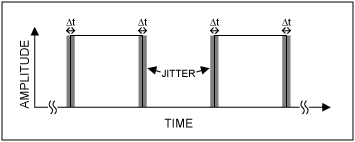
\includegraphics[width=0.5\linewidth]{imagenes/jitter}
	\caption[Ilustración del fenómeno conocido como \textit{jitter}]{En la 
	figura se muestra uan señal digital periódica que presenta pequeñas 
	variaciones en fase. Estas ligeras perturbaciones se conocen como 
	\textit{jitter} y son un efecto no deseado en las señales digitales que 
	provocan funcionamientos erróneos en los sistemas.}
	\label{fig:jitter}
\end{figure}


Dependiendo del tipo de análisis realizado y sobre todo de 
la fuente de ruido que se pretenda caracterizar, será más adecuado trabajar en 
unos casos en el dominio de la frecuencia o en el del tiempo. Sin embargo no 
siempre es posible hacerlo, dado que los aparatos necesarios para muchos de 
estos análisis son bastante caros y es complicado disponer de ellos en el 
laboratorio. \incomment{con esto cubro una posible pregunta para los resultados 
de la cadena de por qué se tomaron con el osciloscopio y no con otra cosa} El 
problema que tiene medir ruido de fase en el dominio del tiempo 
(\textit{jitter}) es el caracter no estacionario del valor RMS del mismo, que 
va creciendo con forme se aumenta el tiempo de medición.

\begin{figure}
	\centering
	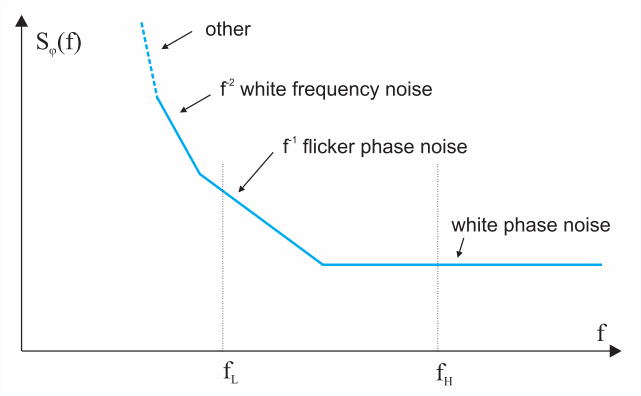
\includegraphics[width=0.7\linewidth]{imagenes/psd_noise}
	\caption[Tipos de ruido en la curva PSD para un XO.]{Clasificación del tipo 
	de ruido según la pendiente de la curva PSD para el ruido de fase de un 
	oscilador}
	\label{fig:psdnoise}
\end{figure}

La entidad IEEE define el término \textit{phase noise} \cite{ieeephysdefs} como 
la mitad 
de la inestabilidad en fase. Donde la inestabilidad en fase ( $S_{\Phi} (f)$ ) 
hace referencia a la densidad espectral de la desviación en fase de la señal. 
Una señal ideal en un oscilador generaría una señal sinusoidal pura, es decir, 
toda la potencia de la señal estaría concentrada en una única frecuencia. Sin 
embargo, esto no sucede en un oscilador real, los cuales tienen componentes de 
ruido moduladas en fase. Típicamente este tipo de medidas se expresa en dBc/Hz, 
indicando la potencia de manera relativa a la frecuencia portadora con un ancho 
de banda de 1Hz. Se utilizan varios desplazamientos con respecto a la 
frecuencia portadora de forma que se puede analizar como afecta el ruido a las 
frecuencias adyacentes a la portadora.

La Figura \ref{fig:psdnoise} muestra los distintos tipos de ruido que se 
identifican por la pendiente de la curva PSD en una doble escala logarítmica. 
En el eje de ordenadas se mide la potencia relativa a la señal portadora en dB, 
y en las abcisas la frecuencia de desplazamiento con respecto a la frecuencia 
portadora. \incomment{si hay tiempo hablar un poco del white noise y otros}

Para obtener este tipo de medidas se necesita equipo bastante caro y preciso. 
Recientemente se ha adquirido en el laboratorio del grupo de sincronización de 
la UGR un medidor de ruido de fase (ver \ref{cap:herram}) que ha posibilitado 
realizar un estudio mucho más detallado que si sólo se hubiese utilizado un 
osciloscopio convencional. Sin embargo, en las primeras fases de este proyecto 
no se contaba con dicho material por lo que se realizan las medidas que fueron 
posibles en ese momento.

\incomment{si hay un poco de tiempo mencionar ADEV y demás tipos y explicar 
rápidamente}


\chapter{Mecanismos de sincronización en redes de computadores}

En este capítulo se detallan las características principales de los mecanismos 
empleados para la sincronización de equipos en red. En concreto se hace 
referencia a tres protocolos, dos que son estándar ampliamente usados, y se 
pueden considerar precursores del tercero, que es en el que se centra este 
trabajo.

Los requisitos demandados por las aplicaciones que necesitan de algún mecanismo 
de sincronización son bastante heterogéneos. Esto es fácilmente entendible si 
se piensa en dos ejemplos de aplicaciones concretos: mantener la hora de 
sistema en los computadores de una red de propósito general, y hacerlo en los 
elementos de una fabrica de montaje de alta precisión.
En ambos escenarios se necesita de un mecanismo que permita mantener una misma 
noción de tiempo en los elementos del sistema, sin embargo en el primer 
escenario se puede tolerar un nivel de error que sería inaceptable en el 
segundo.
En otras aplicaciones, lo realmente importante es que todos los nodos de la red 
realicen una misma cuenta del tiempo, es decir, que la duración de un segundo 
sea lo más parecida en todos los nodos, sin importar tanto la fecha y la hora. 
En estos casos la sincronización se realiza mediante la distribución de una 
señal de reloj que se utiliza en los contadores internos de cada nodo. 

\section{Network Time Protocol}

\textit{\acrlong{ntp}} \cite{Mills1991} es un protocolo estándar de red 
empleado para la sincronización de relojes en computadores conectados mediante 
redes conmutadas, que fue diseñado por David L. Mills de la Universidad de 
Delaware. Su uso se demostró públicamente por primera vez en 1979, en una 
prueba de enlace satelital transatlántico para varios servicios de 
Internet. Posteriormente, en 1985 se implementó NTPv0 para sistemas tipo Unix 
donde la estructura para la cabecera y los cálculos para el tiempo de ida y 
vuelta (o \textit{round-trip time}) y el desfase entre relojes son los que se 
siguen utilizando en la versión actual NTPv4.

Los servidores \gls{ntp} pueden operar en varios modos: \textit{multicast}, 
llamada a procedimiento remoto y simétrico. El modo \textit{multicast} está 
enfocado a redes de área local (\gls{lan}) donde el número de clientes es 
grande y no se necesita de un alto nivel de precisión. En este escenario, uno o 
varios servidores se encuentran continuamente enviando mensajes de difusión 
\gls{ntp} que reciben los clientes que serán los encargados de calcular el 
desfase de su reloj con respecto al del servidor. Los servidores anuncian la 
posibilidad de proveer sincronización pero no aceptan mensajes \gls{ntp} de 
ninguno de los pares.
El segundo modo está pensado para escenarios donde se necesite una gran 
exactitud en la sincronización. Los servidores pueden actuar como cliente 
aceptando la sincronización de otro par (sin proveerla de forma descendente) o 
en modo servidor donde no aceptan ser sincronizados.
Los modos \textit{multicast} y llamada a procedimiento remoto no escalan bien 
en redes grandes de ámbito general como Internet. Para ello, los servidores de 
tiempo deben poder distribuirse de forma dinámica con una topología 
jerarquizada. Para este tipo de modo se emplea la comunicación simétrica donde 
el algoritmo de selección de \gls{ntp} determina el rol de cada uno de los 
servidores en la red.

\subsection{Organización de la red}

La topología de red usada en \gls{ntp} es de tipo jerárquica, donde el índice 
del nivel es un indicativo de la cercanía a la fuente primaria de tiempo. A 
cada nivel de la jerarquía se le denomina estrato. Se comienza a numerar por 0 
y se va sumando 1 por cada nivel de conexión en la jerarquía, es decir, un 
servidor sincronizado a un estrato \textit{n} se encontrará a \textit{n+1} 
saltos de la fuente principal. Este índice indica la distancia a la fuente y no 
necesariamente la calidad del servidor.

\begin{figure}
	\centering
	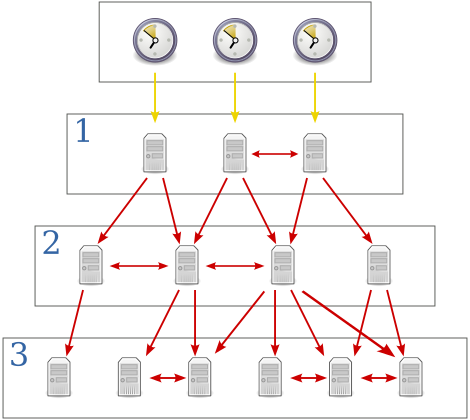
\includegraphics[width=0.7\linewidth]{imagenes/ntp_tree}
	\caption[Esquema de una red de distribución de tiempo usando NTP.]{En este 
	diagrama se 
	muestra una posible red de distribución de tiempo usando NTP. En el estrato 
	0 se hayan las fuentes de reloj de alta estabilidad como GPSDO o relojes 
	atómicos. Estas se conectan directamente a los servidores del estrato 1 que 
	forman los llamados servidores de tiempo primarios. Esta capa provee la 
	hora UTC al resto de los niveles. Como se puede ver, se pueden establecer 
	enlaces entre equipos del mismo nivel, además, pueden estar conectados a 
	varios servidores de la capa superior (redundancia). Imagen tomada de 
	\cite{website:imgNTPtree}}
	\label{fig:ntptree}
\end{figure}


El límite superior para un estrato es el 15. Para indicar que un dispositivo no 
está sincronizado se utiliza el valor de estrato 16. El algoritmo \gls{ntp} 
está diseñado para construir una topología con los caminos más cortos hacía los 
servidores del estrato 1 (haciendo uso del algoritmo Bellman-Ford) lo que 
minimiza el tiempo de ida y vuelta acumulado entre los servidores de estrato 1 
y los clientes. A continuación se describen brevemente los estratos más 
relevantes:

\begin{itemize}
	\item \textbf{Estrato 0} \\ A este nivel se encuentran las fuentes de 
	tiempo de alta precisión, entre las que cabe destacar los relojes atómicos 
	o los osciladores disciplinados por GPS (\acrshort{gpsdo}). Generan una 
	señal de un pulso por segundo (\acrshort{pps}) que permite disciplinar el 
	oscilador interno del servidor conectado a la fuente de nivel 0.
	
	\item \textbf{Estrato 1} \\ Lo forman los servidores cuyos relojes se 
	disciplinan directamente con la señal recibida de una fuente de nivel 0 
	logrando una sincronización en torno a unos pocos microsegundos. Además 
	pueden conectarse con otros del mismo nivel para tareas de comprobación de 
	errores o para redundancia.
	
	\item \textbf{Estrato 2 (en adelante)} \\ Los dispositivos de cada estrato 
	se 
	sincronizan con el estrato anterior, pudiendo hacerlo con varios servidores 
	a la vez, y además con otros computadores del mismo nivel a 
	fin de mejorar la calidad del servicio.
\end{itemize}

\subsection{Algoritmo}

La figura \ref{fig:ntptree} muestra un esquema de organización típico para una 
red de distribución de tiempo usando \gls{ntp}. Para realizar el cálculo del 
desfase del reloj cliente con respecto al servidor, se emplean una serie de 
paquetes con marcas de tiempo (\textit{timestamps}). El cliente debe iniciar el 
proceso realizando una petición al servidor como muestra la figura 
\ref{fig:ntpts}. El servidor recibe el paquete y lo sella en el instante $T_i$. 
Para realizar los cálculos se emplean siempre las 4 marcas más recientes. Con 
ello se puede realizar el cálculo del tiempo de ida y vuelta ($\delta_i$), y el 
desfase del reloj ($\theta_i$) del cliente con respecto al del sevidor en el 
instante de tiempo $T_i$:

\begin{equation}\label{ntprtt}
	\delta_i = (T_{i-2}-T_{i-3}) - (T_{i-1}-T_{i})
\end{equation}\label{ntpoffset}
\begin{equation}
	\theta_i = \frac{(T_{i-2}-T_{i-3}) + (T_{i-1}-T_{i})} {2}
\end{equation}

Hay que tener en cuenta que el servidor no tiene por qué contestar a las 
peticiones del cliente de forma inmediata. El proceso encargado de la gestión 
del servicio \gls{ntp} puede ser interrumpido por otra tarea con más prioridad, 
lo que hace que el tratamiento de las marcas de tiempo no sea determinista.

\begin{figure}
	\centering
	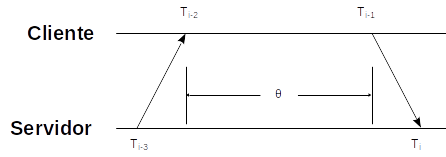
\includegraphics[width=0.7\linewidth]{imagenes/ntp_ts}
	\caption[Cálculo del desfase entre cliente y servidor]{La figura muestra un 
	intercambio de paquetes con marcas de tiempo entre cliente y servidor. Para 
	calcular el tiempo de ida y vuelta se utilizan 4 marcas de tiempo.}
	\label{fig:ntpts}
\end{figure}

\subsection{Rendimiento}

Al ser \gls{ntp} un protocolo que se implementa completamente en 
\textit{software}, no se consigue una gestión determinista para el cálculo del 
desfase entre las dos entidades que se sincronizan. Ello conlleva una 
limitación severa a la precisión alcanzable mediante el uso de este protocolo. 
Aunque este hecho podría ser tratado mediante el 
uso de sistemas operativos de tiempo real o técnicas que consigan reducir la 
latencia con la que el proceso encargado de la gestión del protocolo \gls{ntp} 
es ejecutado, existe otro factor de diseño que tiene incluso más peso en la 
precisión alcanzable por éste: la asunción de igualdad entre los caminos de ida 
y vuelta para los paquetes enviados por la red de comunicación. En \gls{ntp} se 
considera que el camino de transmisión de los paquetes es simétrico al camino 
de recepción, lo cual es bastante improbable en redes conmutadas con varios 
saltos y múltiples caminos como es el caso de Internet. Todo ello conlleva que 
la exactitud que alcanza este protocolo de forma general, sincronizando dos 
equipos, se sitúe en el orden de los milisegundos llegando a decenas de 
microsegundos en condiciones controladas.
\section{Precision time protocol}

Aunque el desarrollo del protocolo \gls{ntp} supuso un gran avance con respecto 
a las técnicas de sincronización en redes utilizadas anteriormente, la 
exactitud que podía alcanzar dicho protocolo no era suficiente para las 
aplicaciones con requisitos de altas prestaciones como los sistemas de control 
o sistemas de medición distribuidos. Para mejorar el rendimiento se propuso el 
desarrollo de un protocolo denominado \acrlong{ptp}, bajo el estándar 
\acrshort{ieee} 1588-2002 (año de su publicación) \cite{IEEE1588-2008}. 
Actualmente se utiliza la segunda revisión del estándar: IEEE 1588-2008 o 
\gls{ptp}v2, que no presenta compatibilidad con la versión anterior.

\subsection{Arquitectura de red}

El protocolo \gls{ptp} define una arquitectura jerárquica de tipo 
maestro-esclavo. Al igual que en la red \gls{ntp}, el nodo raíz puede estar 
conectado a una fuente estable de tiempo, como un \gls{gpsdo} o un reloj 
atómico, y provee de sincronización al resto de la red. En el caso de \gls{ptp} 
este nodo recibe el nombre de \acrlong{gm}. Los nodos intermedios pueden actuar 
como maestros del nivel siguiente o como nodos finales. A continuación se 
detallan las características más relevantes de los tipos de dispositivos más 
usuales:

\begin{itemize}	
	\item \textbf{\gls{oc}} \\
	Este tipo de nodos se comunican con el resto de la red via una única 
	intefaz de red física de tipo bidireccional que se encarga del intercambio 
	de los paquetes con las marcas de tiempo con el resto de la red. La 
	configuración de \gls{oc} sólo permite una única ejecución del 
	protocolo 
	\gls{ptp} y un único estado de funcionamiento. Así, este tipo de 
	configuración, permite al dispositivo actuar como maestro de la red 
	(\acrshort{gm}) o como reloj esclavo.
	
	\item \textbf{\gls{bc}} \\
	Los dispositivos que actúan como \acrshort{bc} suelen disponer de múltiples 
	puertos físicos que pueden actuar como si fuesen \gls{oc}s pero que 
	comparten una misma referencia de tiempo (recuperada del nodo maestro en el 
	nivel superior). Es decir, uno de los puertos se configurará como esclavo y 
	el resto podrán actuar como puertos maestros para los siguientes nodos de 
	la red.
	
	\item \textbf{\gls{tc}} \\
	La gran diferencia con respecto a los tipos anteriores reside en que los 
	\gls{tc} no se sincronizan con un nodo maestro. Estos actúan como simples 
	repetidores del tráfico entrante, pero modifican el campo de corrección de 
	los mensajes \textit{Follow\_UP o Pdelay\_Resp\_Follow\_UP} para incluir el 
	tiempo de residencia de los paquetes \gls{ptp} en el \gls{tc}. El campo de 
	corrección es usado posteriormente por los \gls{oc} para realizar el ajuste 
	de su reloj interno. 
	Dependiendo del mecanismo empleado para el cálculo del tiempo de 
	propagación se distinguen dos tipos de \gls{tc}: \textit{End-to-end} y 
	\textit{Peer-to-peer}.
\end{itemize}

\subsection{Algoritmo}

En el protocolo \gls{ptp} se distinguen dos fases de ejecución:
\begin{enumerate}
	\item Establecimiento de la jerarquía en la red.
	\item Sincronización de los relojes.
\end{enumerate}

En el arranque del algoritmo \gls{ptp} se espera por un lapso de tiempo a 
recibir mensajes de tipo \textit{Announce} provenientes de algún maestro en la 
red. Si no se reciben mensajes de ese tipo, el nodo asume que es maestro hasta 
que un maestro con mejores prestaciones aparezca en la red. La configuración de 
roles en la red se realiza mediante un algoritmo llamado \gls{bmc}, que utiliza 
varios parámetros como calidad de la fuente de reloj de un nodo o el nivel en 
el que se encuentra de la jerarquía (entre otras cosas) para decidir quien debe 
actuar como maestro en la red y quien como esclavo. Este ordenamiento se 
realiza de forma dinámica, de manera que si un nodo se cae, el resto de la red 
se vuelve a configurar en base a los nodos supervivientes.

Tras la fase de establecimiento de la jeraquía se pasa a la fase de 
sincronización, basada en el intercambio de una serie de paquetes 
con marcas de tiempo que permiten al nodo esclavo el cálculo del desfase de su 
reloj con respecto al de referencia en el nodo maestro. El proceso se describe 
en la Figura \ref{fig:ptpts}:

\begin{enumerate}
	\item El maestro manda un mensaje de tipo \textit{Sync} que es sellado 
	temporalmente en base a la escala del maestro en el momento de su envío. 
	Este mensaje puede contener su marca temporal ($T_1$) o necesitar de otro 
	tipo de 
	mensaje (\textit{Follow\_Up}) para transmitirla.
	
	\item El esclavo anota el tiempo de recepción (en su propia escala de 
	tiempo) del mensaje en la marca $T_2$.
	
	\item El esclavo manda un mensaje de tipo \textit{Delay\_Req} al maestro y 
	almacena la marca de tiempo en que lo hace ($T_3$).
	
	\item El maestro sella la recepción del paquete recibido y la envía dentro 
	de un paquete de tipo \textit{Delay\_Resp} ($T_4$).
\end{enumerate}

Una vez el esclavo dispone de las cuatro marcas de tiempo, se procede al 
cálculo del tiempo de propagación en una dirección y del desfase entre relojes 
para poder corregir el reloj en el nodo esclavo.

\begin{equation}\label{delmm}
delay_{mm} = (T_4 - T_1) - (T_3 - T_2)
\end{equation}

\begin{equation}\label{delms}
	delay_{ms} = \frac {1} {2} delay_{ms}
\end{equation}

\begin{equation}\label{offset}
	offset = T_2 - T_1 - delay_{ms}
\end{equation}

Como en el caso de \gls{ntp}, se considera que el tiempo de propagación de los 
mensajes en el camino de ida es igual al de vuelta. En un escenario realista 
esto no tiene por qué cumplirse. Por tanto, cualquier asimetría existente 
introduce un error en el cómputo del valor de desfase.

Los mensajes \gls{ptp} se pueden clasificar dentro de dos clases: mensajes de 
evento y mensajes generales. Todos los mensajes de tipo evento son sellados 
temporalmente tanto en el momento de la emisión como en el de la recepción. 
Dicha marca temporal indica el momento en el que un paquete abandona un nodo y 
entra en el medio de transmisión y viceversa. Con ello se obtienen las 4 
marcas de tiempo necesarias en el cálculo del tiempo de propagación y del 
desfase entre relojes.

Los mensajes de tipo evento son los siguientes:


\begin{itemize}
	
	\item \textbf{Sync} \\
	Es un mensaje transmitido de maestro a esclavo que permite medir el retardo 
	de propagación para un paquete en dicho sentido de la comunicación. Para 
	ello 
	se sella temporalmente el paquete al ser enviado por el maestro y se 
	acompaña dicha marca de tiempo al paquete (o se envía en otro paquete 
	posterior de tipo \textit{Follow\_Up}) para que el nodo esclavo pueda 
	realizar los cálculos. Estos paquetes proporcionan las marcas temporales 
	$T_1 y T_2$.
	
	\item \textbf{Delay\_Req} \\
	Este mensaje lo sella temporalmente el nodo esclavo y lo envía al maestro 
	para obtener la marca temporal de recepción en otro paquete de respuesta 
	denominado \textit{Delay\_Resp}, obteniendo así las marcas $T_3$ y $T_4$, 
	que 
	junto a las dos anteriores permiten calcular el tiempo de ida y vuelta, y a 
	partir de este el desfase de los relojes.
\end{itemize}

En \gls{ptp} se puede medir el retraso producido por la transmisión de los 
paquetes en la red de dos formas distintas. En una modalidad el intercambio de 
paquetes se realiza como muestra la Figura \ref{fig:ptpts}. En ella el cálculo 
del desfase se realiza siempre entre pares de 
dispositivos \gls{ptp} conectados sin tener en cuenta al resto. Esto se 
denomina \textit{end-to-end}.
La otra modalidad consiste en considerar los nodos intermedios entre el nodo 
maestro de la red y el esclavo de turno como si fueran un cable. Para ello, 
los nodos intermedios deben añadir el retardo que supone que los paquetes 
los atraviesen, en un campo del paquete denominado \textit{Correction 
Field}. El esclavo se sincronizará en relación a las marcas de tiempo del 
maestro principal y le sumará los retardos mencionados. A este método se le 
llama \textit{peer-to-peer}.

\textit{Peer-to-peer} tiene la ventaja de no añadir complejidad en el sistema 
ocasionado por varios niveles de dispositivos sincronizándose (encadenar bucles 
de control suele elevar los niveles de ruido del sistema) pero necesita que los 
dispositivos intermedios sean compatibles y sepan modificar el campo 
\textit{correction field}. En caso contrario el nivel de error en la 
sincronización será elevado. El caso de \textit{end-to-end} es más flexible en 
ese aspecto ya que mide el tiempo de ida y de vuelta con el maestro local 
permitiendo corregir mejor los efectos de atravesar dispositivos no compatibles.

Además de los tipos de mensajes listados anteriormente, existen mensajes 
especiales para el modo \textit{peer-to-peer}. Dado que actualmente el protoclo 
\gls{wr} solo implementa comunicación \textit{end-to-end} se omite la 
explicación de los mismos, que puede ser consultada en \cite{IEEE1588_2008}.
En la actualidad se está desarrollando el soporte para \textit{peer-to-peer} y 
\gls{tc}, para más información se puede consultar \incomment{preguntar a JL}.

\begin{figure}
	\centering
	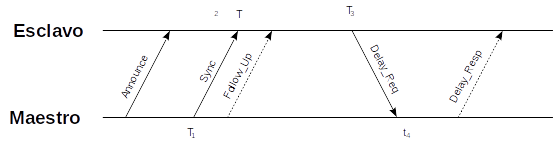
\includegraphics[width=0.7\linewidth]{imagenes/ptp_ts}
	\caption[Intercambio de mensajes para el algoritmo de \acrshort{ptp}]{La 
	figura muestra la secuencia de intercambio de mensajes 
	que se emplea en el algoritmo de \gls{ptp} para conseguir las 4 marcas de 
	tiempo necesarias en el cálculo del \textit{round-trip time} y del desfase.}
	\label{fig:ptpts}
\end{figure}

Para la clase de mensajes generales caben ser destacados los siguientes:

\begin{itemize}
	\item \textbf{Announce} \\
	Es el tipo de mensaje utilizado para informar al resto de los nodos acerca 
	del nodo que transmite (estado y características) además de quién es su 
	\gls{gm}. Son utilizados por el algoritmo \gls{bmc}.
	
	\item \textbf{Follow\_Up} \\
	Sirve para transmitir la marca de tiempo en la escala del maestro para la 
	emisión del mensaje \textit{Sync}.
	
	\item \textbf{Delay\_Resp} \\
	Análogo al anterior para el caso del mensaje \textit{Delay\_Req}.
	
	\item \textbf{Gestión y señalización} \\
	Se engloban mensajes para control y gestión de los relojes o para 
	transmitir información general de estado entre los nodos.
	
\end{itemize}


\subsection{Rendimiento}

Como se ha visto la esencia del mecanismo de sincronización de \gls{ptp} es 
similar al visto anteriormente en la sección de \gls{ntp}: se intercambian una 
serie de paquetes con marcas de tiempo entre dos nodos de la red para calcular 
el desfase entre sus relojes, entonces ¿cómo se consigue la mejora? La gran 
diferencia entre ambos protocolos es la inclusión en el primero del sellado de 
tiempo a nivel de \textit{hardware}. Cuando un paquete de tipo \gls{ptp} llega 
a un puerto, este genera un evento para que una lógica especial realice un 
sellado de tiempo de dicho paquete. Dicha lógica se encuentra entre la capa 
física (PHY) y la capa de enlace (MAC) del modelo \acrshort{osi} 
(\textit{\acrlong{osi}}). Este mecanismo evita la latencia que supone el 
procesamiento de los paquetes y el sellado de tiempo a nivel de 
\textit{software}. Otra diferencia significativa entre \gls{ntp} y \gls{ptp} se 
encuentra en la gestión de las colas de recepción/envío que son fuente de 
retardos no deterministas. Gracias al sellado con soporte \textit{hardware} y 
al tratamiento de los retardos ocasionados por las colas, \gls{ptp} consigue 
una precisión de decenas de nanosegundos con las técnicas más avanzadas 
actualmente. \incomment{referenciar algo}




\section{White Rabbit}

\acrfull{wr} hace referencia tanto al protocolo diseñado como mejora de 
\gls{ptp}v2 como al proyecto internacional que se encarga de su desarrollo y 
mantenimiento. Inicialmente parte como una tecnología desarrollada por el 
\gls{cern} para actualizar el sistema de sincronización y envío de datos de 
control para su complejo de aceleradores de partículas. Gracias a el espíritu 
abierto con el que se desarrolló la tecnología (y a su prometedor rendimiento) 
fueron sumándose otras instituciones al desarrollo, tanto desde el ámbito 
académico, donde cabe destacar el Centro de Investigación de Iones Pesados 
(\textit{Gesellschaft für Schwerionenforschung}, GSI en alemán) en Alemania o 
la propia Universidad de Granada; como desde el empresarial, donde se está 
intentando expandir la tecnología al ámbito industrial. Ejemplos de ello son la 
empresa Seven Solutions (\text{spin-off} de la UGR) en Granada, o CreoTECH en 
Polonia. 

Aunque el empuje en el ámbito de la ciencia es mucho más 
evidente gracias a la inclusión de \textit{WR} en instalaciones para 
aceleradores de partículas, institutos metrológicos o en sistemas de 
adquisición ditribuida como el caso del proyecto Square Kilometre Array (SKA) 
que se está contruyendo en Sudáfrica y que una vez concluido será el 
instrumento de observación astronómica más sensible jamás construido por la 
humanidad. En el caso de la empresa privada, \gls{wr} se ve todavía como una 
tecnología muy prometedora para diversas áreas como Smart Grid, 
Geo-posicionamiento o para las telecomunicaciones, que aún necesita madurar. 
Esto está a punto de cambiar gracias a su inclusión en la próxima revisión del 
estándar \gls{ptp} bajo un nuevo perfil de alta precisión.

Los objetivos de desarrollo iniciales estaban enfocados al entorno de los 
aceleradores de partículas, priorizando una sincronización de calidad junto a 
un sistema que fuese determinista y fácil de mantener:

\begin{itemize}
	\item Lograr para una red de miles de nodos, conectados por enlaces de 
	fibra óptica de hasta 10 km, una diferencia menor del nanosegundo entre dos 
	nodos cualesquiera de la red, es decir, una exactitud de sincronización 
	\textbf{sub-nanosegundo}. Además, se requiere una precisión en el orden del 
	picosegundo.
	
	\item Permitir que el enlace utilizado para los paquetes del protocolo 
	\gls{wr} se pueda \textbf{compartir para} el envío de \textbf{datos de 
	propósito general}, 
	reduciéndo así costes en el despliegue de las infraestructuras.
	
	\item Realizar un desarrollo \textbf{simple y escalable} que no necesite de 
	sofisticados procedimientos de configuración o calibración.
	
	\item Establecer un envío \textbf{determinista} para los paquetes 
	prioritarios, con 
	retardos que no superen ciertos valores umbrales. Esto es especialmente 
	importante en sistemas de control donde la respuesta a un evento no puede 
	exceder un tiempo límite en su envío.
	
	\item Proveer un \textbf{diseño} de referencia \textbf{abierto} a la 
	comunidad 
	(tanto \textit{hardware} como \textit{software}) para fomentar el 
	desarrollo por parte de esta, y evitar las ligaduras con fabricantes.
\end{itemize}

En la actualidad se puede afirmar que en su mayor parte se han cumplido dichos 
objetivos. El requisito principal de rendimiento es algo que se ha conseguido 
en su mayor parte aunque hace falta aportar datos acerca del comportamiento del 
protocolo en redes realmente grandes con un gran número de nodos. La tendencia 
actual en cuanto a rendimiento se centra en la mejora de la exactitud alcanzada 
en escenarios no tan típicos, como enlaces de larga distancia o escenarios con 
cambios en las condiciones de operación. También se investiga como reducir el 
ruido producido por los componentes del sistema de sincronización para lograr 
una precisión en el orden del femtosegundo. El envío determinista es algo que 
no siempre se logra, ya que se puede producir la pérdida de algún paquete de 
alta prioridad en casos de congestión del enlace. Las herramientas de gestión y 
mantenimiento es otro punto al que todavía le queda trabajo por delante y al 
que se está prestando bastante atención dado que son algo crucial si se 
pretende extender el uso del protocolo más allá del ámbito científico.

El protocolo \gls{wr} fue diseñado como una extensión del protocolo IEEE 
1588-2008 (\gls{ptp}v2) al que se añadieron varias mejoras como un modelo de 
enlace más preciso, técnicas de calibración automática o sintonización de los 
relojes mediante el envío de la frecuencia maestra codificada en los paquetes 
transmitidos.

\begin{figure}
	\centering
	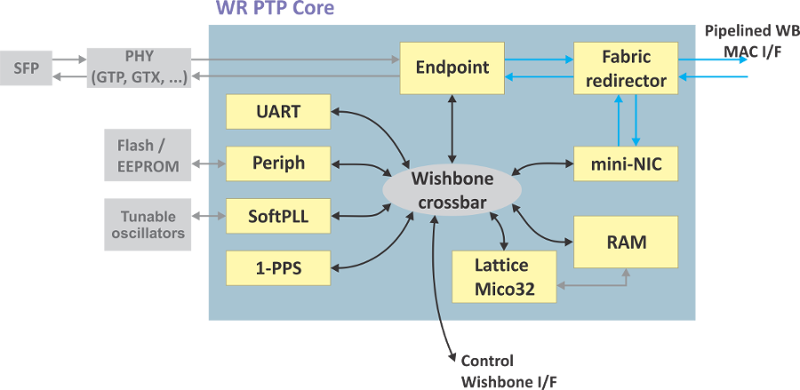
\includegraphics[width=0.7\linewidth]{imagenes/wrpc_inside}
	\caption[Esquema de bloques del WR PTP Core]{En este esquema de bloques se 
	incluyen los componentes principales que componen la arquitectura del WR 
	PTP Core. El bloque principal hace referencia a los componentes en la parte 
	de lógica repogramable, mientras que fuera se incluyen componentes que o 
	bien se incluyen como soporte hw dentro de la FPGA (PHY) o bien son 
	componentes externos que se conectana a algún pin para comunicarse con los 
	elementos internos. Imagen tomada de \cite{Daniluk2012}.}
	\label{fig:wrpcinside}
\end{figure}





\chapter{Análisis limitaciones actuales} \label{cap:cadena}

El proyecto \gls{wr} ofrece dos tipos de arquitectura como referencia: la 
orientada a dispositivos que actúen como \gls{bc}, y la enfocada a nodos 
finales \gls{oc}. En la sección \ref{sec:wr} se ha visto que para la primera se 
cuenta con un dispositivo de referencia, el \gls{wrs}, que implementa la 
arquitectura 
de \gls{bc} y en la cual se centra el desarrollo del \textit{OHWR}. La segunda 
se materializa en la tarjeta \gls{spec} como ejemplo básico de nodo \gls{wr}.

La línea de desarrollo seguida desde la empresa Seven Solutions y desde el 
grupo de investigación enfocado en \gls{wr} de la UGR se ha centrado en el 
desarrollo de las arquitecturas de referencia y en el diseño de nuevos tipos de 
arquitecturas que solucionen las deficiencias presentes en los diseños 
iniciales.

Aunque la estrategía no es la misma si se habla de la arquitectura de 
\textit{switch} que si se hace de la de nodo, si es cierto que hay una 
corriente que se comparte en ambos desarrollos: la utilización de los nuevos 
modelos de \gls{soc} para lograr un mayor nivel de integración y un aumento de 
las prestaciones del sistema sin elevar la complejidad del mismo en exceso.

En el caso del \gls{wrs} existente se han detectado varios problemas por la 
gran complejidad del diseño \textit{hardware} que tiene el circuito 
electrónico. 
Uno de ellos es la comunicación entre el procesador ARM y el circuito  
implementado en la lógica reconfigurable de la \gls{fpga}. Gracias a la mejora 
en la 
tecnología de fabricación se consiguen actualmente sistemas que integran tanto 
\gls{fpga} como microprocesador en un único chip reduciendo costes y 
complejidad de desarrollo.

La arquitectura referencia para los nodos \gls{wr} ha tratado de ofrecer un 
diseño básico y asequible económicamente. El uso de la familia Spartan de 
Xilinx ha permitido mantener los costes bajos a la vez que ha permitido alojar 
el diseño básico de la arquitectura de nodo \gls{wr} . Sin embargo, dicho 
diseño se está mejorando y está recibiendo cada vez más funcionalidades por lo 
que la necesidad de recursos está creciendo. Además, dicho diseño tiene una 
limitación bastante importante: carece de un microprocesador dedicado lo que 
dificulta en gran medida el desarrollo e incorporación de nuevas 
características. De igual forma que en la arquitectura de \textit{wrs} se 
tiende hacía soluciones en \gls{soc}, la arquitectura de nodo se puede 
beneficiar de este tipo de soluciones ya que permiten incluir un 
microprocesador físico en el diseño sin necesidad de gastar puertas para 
incluirlo y además mantener los costes bajos.

Mi trabajo de investigación se ha enfocado en la arquitectura de nodo por lo 
que será a la que haga referencia en el resto de la memoria, aunque como he 
comentado en los párrafos anteriores, muchas de las mejoras planteadas a 
continuación se pueden incorporar en la arquitectura tipo \textit{switch}.

El primer paso para poder plantear mejoras a la arquitectura de nodo y al 
rendimiento de la sincronización en los mismos es establecer el punto de 
partida. Para ello se ha realizado una labor de análisis de una arquitectura 
actual de nodo basada en un diseño similar al de la tarjeta SPEC pero 
que ya presenta una serie de mejoras.

El nodo utilizado como punto de partida es el WR-LEN \cite{website:len}. Dicho 
dispositivo incorpora una versión 
mejorada del \gls{wrc} denominado \gls{wrc2p} cuya principal característica es 
la inclusión de un segundo puerto físico a la arquitectura de nodo.

\subsection{White Rabbit Core Dual Port}

El \gls{wrc2p} \cite{felipe16} es una extensión de la arquitectura para nodos 
\gls{wr} 
denominada \acrlong{wrc} \cite{Daniluk2012} que añade una segunda interfaz 
física 
Ethernet a la arquitectura básica mono-puerto. En la implementación actual, la 
referencia temporal es única para ambos puertos, lo que supone que el 
dispositivo puede actuar como nodo (esclavo o maestro) y como \gls{bc}, es 
decir, esclavo de un nivel superior de la jerarquía de red y maestro de un 
nivel inferior. Además, se pretenden desarrollar técnicas que habiliten la 
redundancia (hacer un cambio de referencia si un enlace se cae).

Esta nueva arquitectura de nodo extendida permite el desarrollo de dispositivos 
\gls{bc} de coste reducido que son ideales para su uso en topologías lineales, 
donde el uso de \gls{wrs}s supone una infrautilización de los puertos 
disponibles por equipo.

\begin{figure}
	\centering
	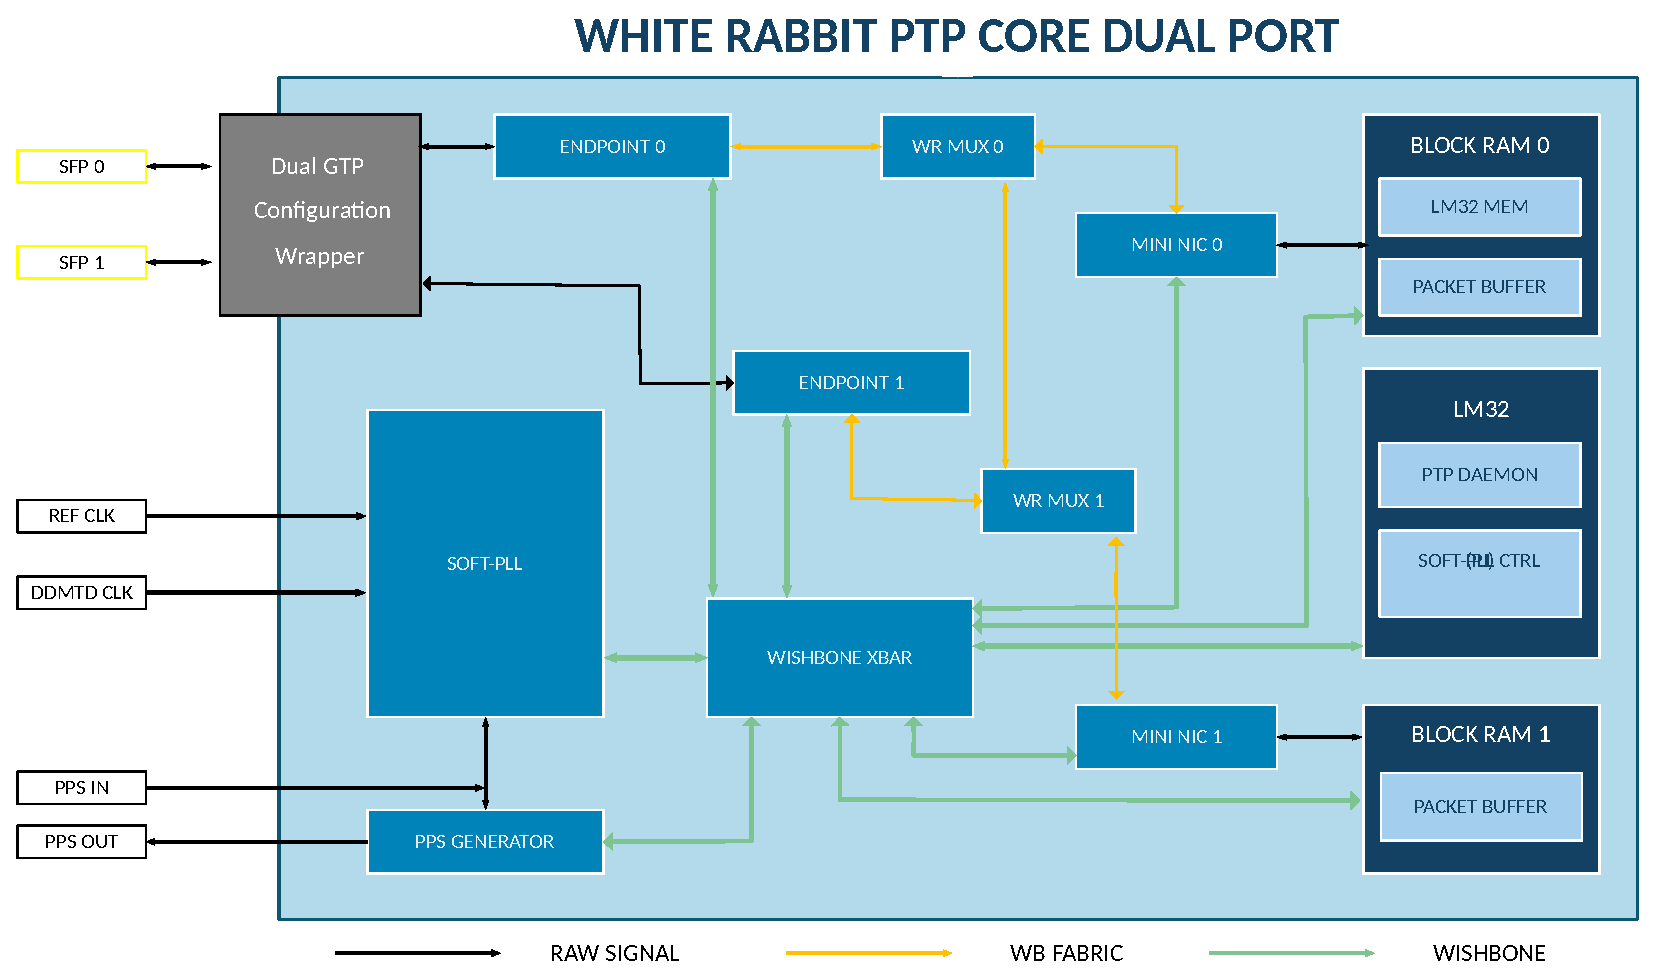
\includegraphics[width=\linewidth]{imagenes/wrpc_dp}
	\caption[Diagrama de bloques del WRC2P]{Este diagrama muestra la estructura 
	de módulos HDL para el diseño de la arquitectura WRC2P.}
	\label{fig:wrpcdp}
\end{figure}


La Figura \ref{fig:wrpcdp} muestra como se organizan los módulos para la 
arquitectura de \gls{fpga}. Con respecto al diseño de referencia se realiza una 
duplicación de los componentes principales de la lógica de \gls{wr}: 
\textit{endpoint}, multiplexor WR, mini-NIC
y los módulos de RAM. Sin embargo el bloque para el procesador embebido se 
mantiene, realizando únicamente cambios a nivel de \textit{sw}. Con ello se 
consigue reducir el número de puertas necesarias, algo clave para alojar la 
arquitectura dentro de una FPGA de perfil bajo.

\subsection{WR-LEN}

El WR-LEN es el primer dispositivo \gls{wr} en incorporar la arquitectura 
\gls{wrc2p}. Sus principales características son la inclusión de un segundo 
puerto físico compatible con \gls{wr}, conectores coaxiales de tipo \gls{sma} y 
una tercera interfaz Ethernet de tipo 1000BaseT.

\begin{figure}
	\centering
	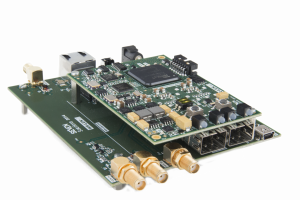
\includegraphics[width=0.7\linewidth]{imagenes/wrlen}
	\caption[WR-LEN en su versión para desarrolladores]{Imagen de un equipo 
	WR-LEN sin caja. Se puede observar como se compone de dos tarjetas: la 
	principal (arriba) donde se sitúa la electrónica de control de WR, y el 
	\textit{backplane} (abajo) que dota de interfaces de entrada/salida a la 
	primera.}
	\label{fig:wrlen}
\end{figure}


La electrónica encargada de la recuperación de reloj y mantenimiento de la 
referencia de tiempo local se mantiene con respecto a la utilizada en el 
\gls{wrs}. El oscilador principal es un modelo que compensa el cambio de 
temperatura y permite el ajuste de la frecuencia por medio de voltaje (VCTCXO) 
Mercury VM53S3. También se ha mantenido el \gls{pll} que se encarga de generar 
las frecuencias necesarias para la lógica de control de WR es el AD9516-4 de 
Analog Devices. Un cambio reseñable se encuentra en el reloj utilizado 
para los módulos 
\gls{ddmtd} que ya no utiliza un \gls{pll} externo para generar la frecuencia 
de 62.5 MHz necesaria, si no que se aprovecha uno de los \gls{pll} internos de 
la \gls{fpga} para ello.

\subsection{Experimentos de escalabilidad}

Para evaluar las limitaciones del \gls{wrc2p} en cuanto a prestaciones y 
escalabilidad realicé una serie de experimentos encadenando múltiples nodos 
\gls{wr} \cite{felipe16}. A través del análisis de la señal de reloj de salida 
producida por 
la lógica de \gls{wr} se pueden obtener indicadores de como de estable es el 
proceso de sincronización en cada nodo, o dicho de otra forma, cuanto ruido 
electromagnético se añade a la señal fundamental de \gls{wr} por cada salto. La 
hipótesis de partida es que debido al ruido electromagnético y demás fuentes 
posibles de inestabilidad debe de existir un número máximo de nodos 
sincronizables bajo las condiciones de exactitud de WR, es decir, en algún 
momento se perderá el sub-nanosegundo. Además, si el aumento del nivel de ruido 
es alto, llegará un momento en el que ni siquiera sea posible sincronizar, 
debido a que la frecuencia recuperada del enlace esté fuera de rango para el 
bucle de control que disciplina el oscilador del nodo. Para comprobar dichas 
hipótesis se han propuesto una serie de experimentos cuyos resultados deben 
permitir establecer los límites de la implementación 
(comprobar si se cumple la exactitud sub-nanosegundo) y detectar las 
deficiencias o mejoras posibles a fin de mejorar el diseño existente.

\begin{figure}
	\centering
	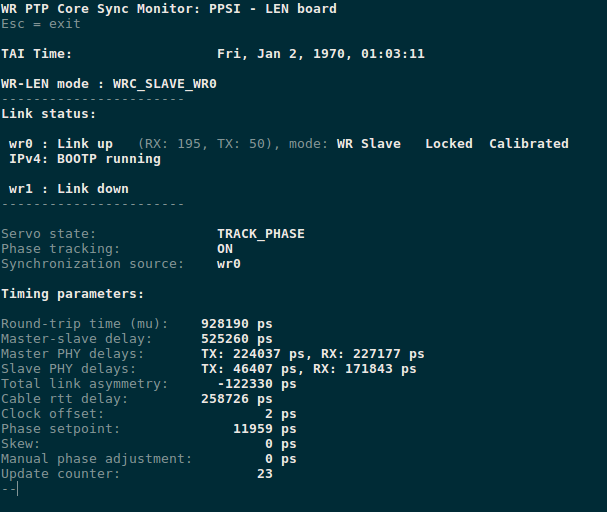
\includegraphics[width=0.7\linewidth]{imagenes/len_gui}
	\caption[Captura del monitor WR en el dispositivo WR-LEN]{Esta captura 
	muestra la información que aporta el monitor interactivo WR para el caso de 
	un nodo. Los datos más importantes son los relativos a la hora del sistema, 
	el modo de operación y el estado del servo. Además se ofrecen estadísticas 
	del enlace como el \textit{round-trip time} o la asimetría.}
	\label{fig:lengui}
\end{figure}


De las alternativas disponibles en el universo de los dispositivos WR, se ha 
utilizado la arquitectura basada en nodo, y en concreto 
WR-LENs para realizar este tipo de pruebas: por un lado, los resultados 
obtenidos se pueden extrapolar a otros diseños como el del \gls{wrs}. Esto se 
debe a que el mecanismo de sincronización es prácticamente el mismo en ambas 
arquitecturas. Y por el otro, está el sentido práctico: realizar una cadena de 
muchos equipos es complejo en cuanto a la gran necesidad de material y recursos 
en el laboratorio. El uso de equipos simples como el WR-LEN ha hecho posible 
llegar a conectar un elevado número de nodos en cascada (hasta 18) permitiendo 
así observar el comportamiento de la tecnología en una red con un gran número 
de saltos (o \textit{hops}).

El primer experimento está pensado para comprobar si efectivamente la 
sincronización se deteriora hasta el punto de no lograr sincronizar un equipo 
(aunque sea fuera del nanosegundo de diferencia).
Para ello se desplegó una red de WR-LEN conectadas en cadena, tal como muestra 
la Figura \ref{fig:chainschema}. Para comprobar la exactitud de la 
sincronización en los puntos elegidos, se toma el reloj de salida del nodo 
maestro como referencia y el reloj del nodo esclavo i-ésimo, y con la ayuda de 
un osciloscopio de alta resolución se toman muestras de la diferencia en el 
dominio del tiempo entre los flancos de subida de las señales de reloj o de los 
PPSs.

Antes de efectuar las pruebas es necesario realizar una calibración de los 
retardos de propagación típicos de los dispositivos WR-LEN necesarios por el 
modelo de enlace para el cálculo del desfase. También hace falta calcular el 
coeficiente de asimetría relacionado con la diferencia de velocidad de 
propagación entre la señal empleada para transmitir y la de recibir. El 
procedimiento para dicho proceso de calibración se encuentra descrito en 
\cite{man:calib}. Los valores obtenidos pueden reutilizarse entre dispositivos 
que mantengan la misma versión de \textit{firmware}. Reutilizar dichos valores 
conlleva una pequeña pérdida de exactitud dado que no se tienen en cuenta las 
pequeñas variaciones que existen entre tarjetas, cosa que puede parecer 
insignificante pero que toma relevancia cuando hablamos de cotas de 
sincronización que alcanzan las decenas de picosegundos de exactitud. Sin 
embargo no se ha considerado necesario llegar hasta estos extremos ya que el 
resultado principal que se pretende obtener son los valores relativos a la 
precisión, es decir, como de estable son las señales producidas por los 
dispositivos. Así pues se observarán pequeños desplazamientos en las medidas de 
desfase entre las señales de maestro y esclavo, que se irán acrecentando con 
forme se aumente el número de nodos en cascada.

Para comprobar si un nodo logra sincronizarse, además de observar las señales 
de salida, se debe consultar el monitor de estado de \textit{wr}. En la Figura 
\ref{fig:lengui} se incluye una captura de dicho monitor. Como se ha 
mencionando anteriormente, este primero experimento busca 
determinar en que momento un nodo es incapaz de sincronizarse con el resto de 
la red. Para determinarlo, se debe ir conectando uno a uno cada dispositivo y 
comprobar el estado de la sincronización es \textit{Track-Phase}. 
Además se puede ir comprobando que la diferencia en tiempo entre las señales de 
\gls{pps} del maestro \textit{free-running} y de cada nodo sea inferior al 
nanosegundo. Las pruebas se han tomado por período de una hora y cada 
experimento se ha repetido tres veces para comprobar la consistencia de los 
resultados.

\begin{figure}
	\centering
	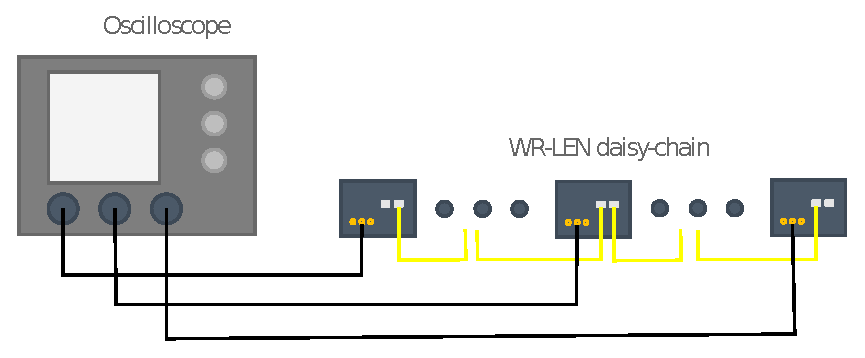
\includegraphics[width=0.7\linewidth]{imagenes/chain_schema}
	\caption[Esquema de conexión para los experimentos de escalabilidad.]{El 
	esquema muestra como se han conectado los diferentes nodos que han 
	compuesto la red WR para los experimentos de escalabilidad. Cada nodo actúa 
	como esclavo del nivel inferior y como maestro del siguiente (cascada).}
	\label{fig:chainschema}
\end{figure}

\begin{table}
	% increase table row spacing, adjust to taste
	\renewcommand{\arraystretch}{1.3}
	% if using array.sty, it might be a good idea to tweak the value of
	% \extrarowheight as needed to properly center the text within the cells
	\caption{Medidas de desfase para el primer experimento de la cascada de 
	WR-LEN con 18 nodos.}
	\label{tab:cascada1}
	\centering
	% Some packages, such as MDW tools, offer better commands for making tables
	% than the plain LaTeX2e tabular which is used here.
	\begin{tabular}{|c||c||c||c|}
		\hline
		Desfase & Mean & $\sigma$ & peak-to-peak \\
		\hline
		Maestro al 10º nodo & -212.51 ps & 45.653 ps & 312.50 ps \\
		\hline
		Maestro al 15º nodo & -500.66 ps & 174.50 ps & 1.0731 ns \\
		\hline
		Maestro al 18º nodo & -573.45 ps & 490.17 ps & 2.6487 ns \\
		\hline
	\end{tabular}
\end{table}

En el contexto de este análisis los valores más relevantes extraídos son los 
correspondientes a la desviación típica y al llamado \textit{peak-to-peak} que 
no es más que la diferencia entre el valor máximo y el mínimo. Con el primero 
nos podemos hacer una idea del ruido presente en el sistema y con el segundo se 
comprueba cuando, en el peor de los casos, la sincronización pierde en algún 
momento el nanosegundo de exactitud. ¿Por qué no interesa el valor medio? Al 
principio de la sección se ha mencionado que se han utilizado los mismos 
parámetros de calibración para todos los nodos. Esto es algo típico y que 
funciona bastante bien cuando nos encontramos dentro de un escenario usual de 
red. Sin embargo, es totalmente posible realizar una calibración por nodo 
consiguiendo así que el valor medio esté centrado en 0. Dado que el foco de 
este análisis es el ruido y sus consecuencias, no se ha considerado relevante 
invertir tiempo en realizar un proceso de calibración completo que habría 
supuesto invertir mucho tiempo.

Los resultados numéricos de este primer experimento se incluyen en la Tabla 
\ref{tab:cascada1} y también se puede observar la distribución que siguen las 
muestras tomadas en la Figura \ref{fig:histexp1}. Se incluyen únicamente los 
resultados en los nodos 10º, 15º y 18º por motivos de reproducibilidad del 
experimento. Dado que el osciloscopio cuenta con 4 canales de entrada y uno de 
ellos es el utilizado por la referencia, solo se pueden tomar al mismo tiempo 
medidas de 3 nodos.
Del montaje inicial de la red se determinó que la sincronización 
sub-nanosegundo se consigue hasta el nodo 12º. Aunque los siguientes nodos se 
encuentran \textit{en media} dentro de rango, el análisis del peor de los casos 
muestra que es a partir del nodo 12º cuando no se puede asegurar que la 
diferencia entre la marca temporal del maestro y la del nodo sea siempre menor 
del ns \textit{explicar como se calcula eso que no es trivial}. Aún así los 
valores medios pueden ser interesantes para aplicaciones 
que no sean críticas y permitan cierta tolerancia a este fenómeno.
El otro resultado importante al que se llegó fue que a partir del nodo 18º no 
se consigue pasar de la fase de sintonización por lo que \gls{wr} no puede 
funcionar. Es decir, se comprobó que la hipótesis era cierta y el incremento 
del nivel de ruido por salto ocasiona un deterioro constante de la distribución 
de tiempo que llega hasta el punto de ser imposible sincronizar sin realizar 
ajustes en el algoritmo de control para relajar las condiciones del bucle de 
control.

Tras observar ambos resultados, se realizó una toma de medidas de desfase entre 
nodos clave: 10º, 15º y 18º. Los primeros nodos mostraban valores bajos de 
ruido por lo que resultaba más interesante analizar que pasaba cerca del punto 
donde se pierde la sincronización y al final de la cadena, donde el ruido 
comienza a ser muy elevado. Los resultados mostrados en la Tabla 
\ref{tab:cascada1} ayudan a comprender que falla para que a partir del nodo 18º 
no se consiga sintonizar. El problema se debe a el alto nivel de ruido en la 
señal que se recupera del enlace y que por tanto se sale de los límites que 
permite el bucle de control encargado de medir el desfase y disciplinar el 
reloj local. Para solucionar este problema se puede aumentar el ancho de banda 
de dicho bucle para permitir cambios más grande en frecuencia de la señal 
recuperada. Esto tiene una repercusión y es que se aumenta el nivel de ruido 
del sistema debido a que el filtro formado por el bucle de control reacciona a 
un mayor ancho de banda siendo vulnerable a perturbaciones no deseadas en la 
señal de reloj. 



Otro de las pruebas realizadas busca comprobar una de las hipótesis del procolo 
WR de que la longitud 
del enlace de fibra óptica no tiene un efecto considerable sobra la precisión 
de la sincronización (siempre considerando una longitud dentro del rango de 
operación de los \gls{sfp}s utilizados). Para ello se replicó el montaje en 
cadena, pero utilizando menos nodos (15) pues los valores de los nodos finales 
en cadenas largas son muy inestables y aportan poca confianza estadística a la 
hora de determinar si hay diferencia o no entre usar un enlace corto o no. Las 
medidas de desfase se han tomado en los nodos 13º, 14º y 15º, usando un enlace 
de 5 km entre los nodos 13º y 14º.

\begin{table}
	% increase table row spacing, adjust to taste
	\renewcommand{\arraystretch}{1.3}
	% if using array.sty, it might be a good idea to tweak the value of
	% \extrarowheight as needed to properly center the text within the cells
	\caption{Medidas de desfase para el segundo experimento de la cascada de 
		WR-LEN usando fibras cortas.}
	\label{tab:cascada2}
	\centering
	\begin{tabular}{|c||c||c||c|}
		\hline
		Desfase & Mean & $\sigma$ & peak-to-peak \\
		\hline
		Maestro al 13º nodo & -368.82 ps & 117.08 ps & 694.23 ps \\
		\hline
		Maestro al 14º nodo & -367.75 ps & 173.45 ps & 971.43 ps \\
		\hline
		Maestro al 15º nodo & -766.19 ps & 235.77 ps & 1.373 ns \\
		\hline
	\end{tabular}
\end{table}

\begin{table}
	% increase table row spacing, adjust to taste
	\renewcommand{\arraystretch}{1.3}
	% if using array.sty, it might be a good idea to tweak the value of
	% \extrarowheight as needed to properly center the text within the cells
	\caption{Medidas de desfase para el segundo experimento de la cascada de 
		WR-LEN usando un enlace de 5 km entre los nodos 13º y 14º.}
	\label{tab:cascada3}
	\centering
	% Some packages, such as MDW tools, offer better commands for making tables
	% than the plain LaTeX2e tabular which is used here.
	\begin{tabular}{|c||c||c||c|}
		\hline
		Desfase & Mean & $\sigma$ & peak-to-peak \\
		\hline
		Maestro al 13º nodo & -341.08 ps & 101.02 ps & 507.05 ps \\
		\hline
		Maestro al 14º nodo & -271.06 ps & 234.52 ps & 859.52 ps \\
		\hline
		Maestro al 15º nodo & -700.65 ps & 203.93 ps & 1.5425 ns \\
		\hline
	\end{tabular}
\end{table}

Los resultados se incluyen en la Tabla \ref{tab:cascada2} para el caso de todos 
los enlaces con fibras cortas, y en la Tabla \ref{tab:cascada3} para el del 
enlace de varios kilómetros. Al igual que para el primer experimento se 
incluyen los histogramas de la distribución de las muestras en las Figuras 
\ref{fig:histexp2} y \ref{fig:histexp3} respectivamente. La diferencia 
observada entre los dos experimentos muestra que no hay diferencia 
significativa (los valores tienen una gran dispersión) entre el uso de un 
enlace de varios kilómetros o uno casi despreciable, tanto en el caso del nodo 
conectado con el enlace como en el siguiente. Además los resultados son 
consistentes con lo visto en el primero experimento: el nodo 13º se encuentra 
fuera (por poco) del ns en el peor de los casos, y el nodo 15º presenta una 
dispersión en torno a los 200 ps.

\begin{figure}
	\centering
	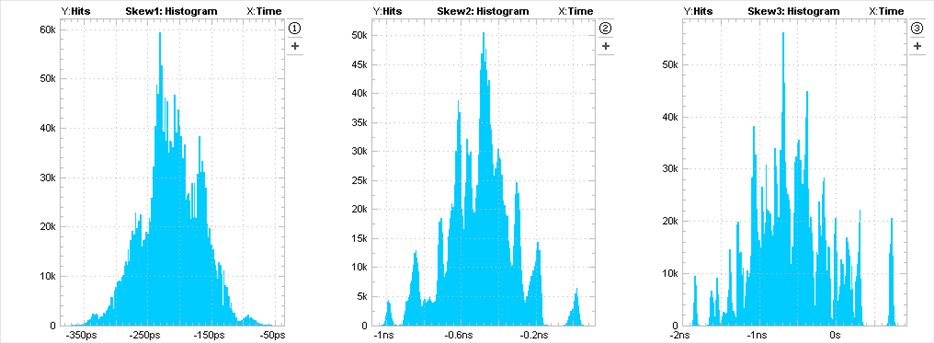
\includegraphics[width=0.7\linewidth]{imagenes/hist_exp1}
	\caption[Histograma para cadena de 18 WR-LEN]{Los histogramas muestran la 
	distribución de las muestras correspondientes a la diferencia entre las 
	señales de PPS en el maestro y la de los nodos 10, 15 y 18.}
	\label{fig:histexp1}
\end{figure}

\begin{figure}
	\centering
	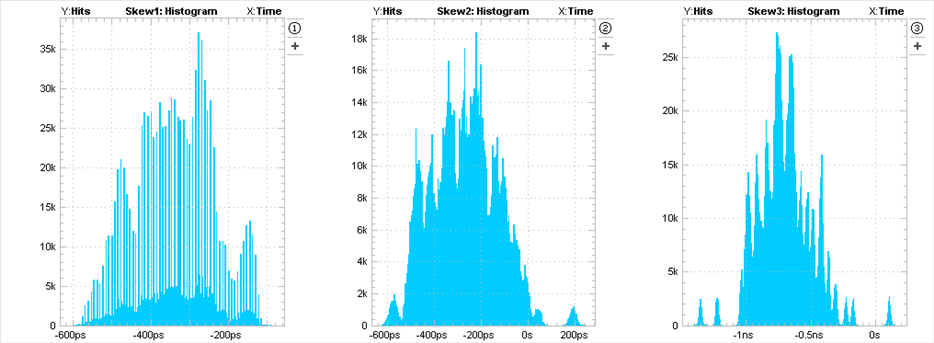
\includegraphics[width=0.7\linewidth]{imagenes/hist_exp3}
	\caption[Histograma para cadena de 15 WR-LEN]{Los histogramas muestran la 
		distribución de las muestras correspondientes a la diferencia entre las 
		señales de PPS en el maestro y la de los nodos 10, 15 y 18.}
	\label{fig:histexp2}
\end{figure}

\begin{figure}
	\centering
	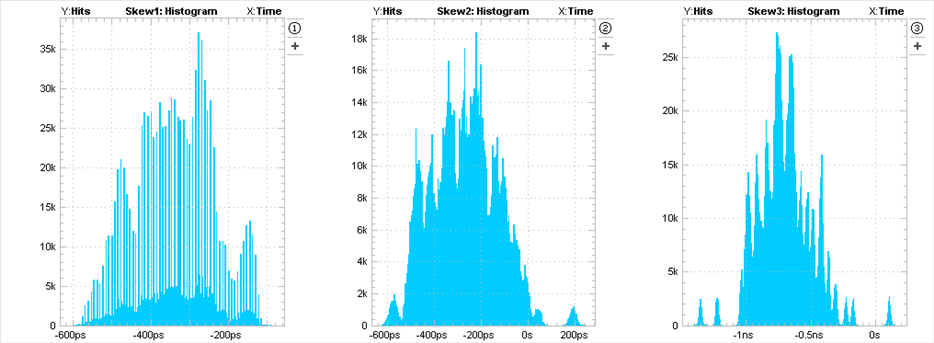
\includegraphics[width=0.7\linewidth]{imagenes/hist_exp3}
	\caption[Histograma para cadena de 15 WR-LEN con un enlace de 5km]{Los 
	histogramas muestran la distribución de las muestras correspondientes a la 
	diferencia entre las señales de PPS en el maestro y la de los nodos 10, 15 
	y 18.}
	\label{fig:histexp3}
\end{figure}

\subsubsection{Conclusiones}

Los experimentos realizados sobre una red de dispositivos \gls{wr} conectados 
en cascada han arrojado varios resultados interesantes y han permitido 
comprobar las hipótesis acerca del efecto del ruido en el sistema y us 
consecuencias:

\begin{itemize}
	\item Se ha realizado una caracterización de la implementación \gls{wrc2p}, 
	la cual extiende la funcionalidad de la arquitectura clásica de nodo 
	\gls{wr} manteniendo un diseño alojable en \gls{fpga}s de perfil bajo. Dado 
	que dicha implementación es relativamente nueva, era importante comprobar 
	que el nuevo diseño cumple las especificaciones básicas del protocolo  
	\gls{wr} antes de trabajar en las posibles mejoras.
	
	\item Se han obtenido resultados muy interesantes en cuanto a los límites 
	de la tecnología, observando que no se consiguen sincronizar más de 18 
	equipos en cadena. Este tipo de pruebas no se había realizado hasta la 
	fecha con un número tan elevado de equipos \gls{wr} por lo que dichos 
	resultados son de gran utilidad para el resto de la comunidad. Si bien los 
	resultados se han obtenido usando equipos de bajo perfil, la electrónica de 
	control es en su mayor parte idéntica a la usada por el \gls{wrs} por lo 
	que se puede extrapolar las conclusiones pensando que quizás en el caso de 
	una cadena de 18 \gls{wrs}s se podría obtener cierta mejora gracias a 
	contar con una \gls{fpga} de perfil alto que cuenta con 
	\textit{transceivers} GTX en lugar 
	de GTP.
	
	\item Se ha comprobado la hipótesis de que gracias al nuevo modelo de 
	enlace presente en \gls{wr} se consigue calibrar de forma dinámica la 
	longitud del enlace de fibra óptica mediante la utilización del parámetro 
	de asimetría.
\end{itemize}

Además he podido comprobar de primera mano que aspectos son mejorables y la 
posible línea de trabajo futuro. En cuanto a la arquitectura de nodo, he 
detectado una serie de problemas que merece la pena discutir. En primer lugar, 
hay que entender ciertas decisiones del diseño inicial que se pudieron tomar 
para realizar un sistema que fuera sencillo y mantuviese los costes bajos. Con 
esto me refiero a la ausencia de un microprocesador físico externo que permita 
obtener un mayor rendimiento y flexibilidad de desarrollo para el \textit{sw} 
de la plataforma. El código \textit{sw} actual de un nodo se ejecuta en 
procesador embebido, el LM32. Este, cuenta con unos recuros muy limitados y se 
nota 
bastante a la hora de desarrollar para esta plataforma. Al incorporar una 
\gls{fpga} de perfil bajo, el número de recursos disponibles es limitado: hay 
pocas puertas lógicas disponibles y el número de bloques de memoria RAM es 
bajo. Eso provoca que el rendimiento de ejecución del LM32 sea bastante bajo y 
el desarrollo de nuevas características está limitado por la falta de recursos. 
Hay que tener en cuenta que este sistema se pensó en un primer momento para 
gestionar una única interrupción del \textit{Soft-PLL} y realizar el cálculo 
del desfase en tiempo real. Es el caso del \gls{wrs}, donde la única función 
del LM32 es esa. En el desarrollo de la arquitectura de nodo, al carecer de un 
procesador físico disponible, se tuvo que incluir en el \textit{sw} embebido 
del LM32 todos los programas de interfaz con el usuario, el demonio \gls{ptp} y 
cualquier característica que no se implementa en HDL. Con forme el diseño ha 
ido aumentando en complejidad, la sobrecarga de este procesador se ha hecho 
evidente, llegando al punto de que el actual diseño del \gls{wrc2p} incluido en 
la WR-LEN no permite incluir ninguna funcionalidad extra por falta de memoria 
RAM y de capacidad de cómputo. También cabe mencionar el poco soporte para 
depuración que presenta este tipo de sistema, llevando mucho más tiempo 
desarrollar en esta plataforma que, por ejemplo, en un ARM.

Las herramientas de gestión incluidas en la WR-LEN son muy básicas y han hecho 
bastante laborioso realizar los experimentos con tantos nodos al mismo tiempo. 
Una vez más, debida a la falta de un SO o de una plataforma más estandarizada, 
desarrollar cualquier herramienta de control ha llevado bastante tiempo y 
actualizar el sistema no es algo trivial.

Gracias a los avances recientes en los procesos de fabricación de circuitos 
integrados actualmente podemos disponer de sistemas que integran varios 
componentes en un único chip, incluyendo una FPGA y un procesador físico en un 
mismo integrado a la vez que se mantiene un coste bajo. Como la mayoría de los 
diseños WR se basan en FPGAs de Xilinx, se puede pensar en la familia Zynq-7000 
de este fabricante como mejora a la arquitectura existente de nodo. De esta 
forma se puede incluir un SO tipo Linux que se integre de forma 

Esta nueva propuesta de plataforma se propone con más detalle en el siguiente 
capítulo, hablando de la línea de desarrollo actual y de los pasos futuros.



\chapter{Arquitectura de nodo basada en SoC}

En el capítulo anterior se han motivado el por qué de un cambio de arquitectura 
para el diseño de los nodos WR: aumento de la capacidad de cómputo, desarrollo 
de herramientas \textit{sw} más rápido y fácil, posibilidad de la inclusión de 
un SO, etc. Además gracias a las nuevas familias de SoC desarrolladas, ello no 
conlleva elevar en exceso el coste de fabricación del dispositivo. 
En este capítulo se discute la línea de trabajo e investigación actual para el 
desarrollo de nodos basados en SoC. Se explican los cambios necesarios para 
realizar una traslación del diseño actual del \gls{wrc2p} de la familia Artix-7 
(FPGA pura) a la familia Zynq-7000 (FPGA+ARM). Al final del capítulo se discute 
que línea se va a seguir en el futuro con motivo de aprovechar al máximo los 
recursos de la nueva plataforma basada en SoC y las posibles mejoras a la 
implementación inicial realizada para este tipo de plataforma.

\section{Características del diseño basado en SoC para Xilinx}

El diseño basado en SoC permite elevar el nivel de abstracción a la hora de 
definir los componentes que integrarán el sistema final. En concreto los SoC 
que incluyen FPGAs tienen la ventaja de ofrecer la flexibilidad de un sistema 
basado en FPGA (\textit{hardware} reconfigurable) con el rendimiento de los 
circuitos dedicados a tareas específicas, como un procesador de propósito 
general, un procesador digital de señales (DSP), interfaces de bus serie, 
controladores de memoria, y un largo etcétera. Cada fabricante suele ofrecer 
una serie de familias o gamas de productos en esta línea que se diferencian por 
los componentes físicos incluidos en el SoC y por las características de la 
FPGA. Para el caso que nos ocupa de desarrollo de un nodo WR, las 
características principales que debe poseer un SoC son:

\begin{itemize}
	\item Núcleo de lógica programable (FPGA). Obviamente toda la lógica 
	implementada en VHDL del núcleo WR se necesita implementar como 
	\textit{hardware} reconfigurable en una FPGA. Los requisitos de esta no son 
	demasiado exigentes ya que el diseño heredado ya estaba funcionando en una 
	FPGA de perfil bajo como la familia Spartan.
	
	\item Microprocesador de propósito general. Dadas las características 
	actuales de los nodos basados en FPGA con el LM32, cualquier core ARM de 
	los incorporados en los SoC de perfil bajo es suficiente para ofrecer la 
	capacidad de cómputo necesaria para este tipo de aplicaciones.
	
	\item Transceiver \incomment{rellenar}
	
	\item Interfaces DMA \incomment{rellenar}
	
	\incomment{pensar en más mierdas}
\end{itemize}

Con estos requisitos la familia Zynq-7000 encaja perfectamente tanto a la hora 
de cumplir los requisitos marcados anteriormente como en la de mantener un 
coste reducido. Los componentes principales de esta familia son los siguientes:

\begin{itemize}
	\item Microprocesador ARM Cortex-A9 de doble núcleo.
	\item Parte de lógica programable equivalente a un modelo Artix-7 (misma 
	familia que incopora el WR-LEN).
	\item Controlador de memoria con soporte para DDR3.
	\item Controlador \gls{dma} hacía módulos RAM externos.
	\item Ethernet MAC configurable a 10/100/1000 
\end{itemize}


\subsection{Arquitectura de la Familia Zynq-7000}
\incomment{arquitectura zynq-7, hablar un poco de los recursos y de como se 
organizan los componentes}

\subsection{Herramientas de desarrollo de Xilinx}
\incomment{hablar del nuevo modelo de trabajo basado en vivado y las cajitas}

\section{Migración y desarrollo de una arquitectura de nodo basada en SoC}

El llamado \textit{\acrlong{wr} Zynq Embedded Node} (WR-ZEN) es la primera 
plataforma que incorpora la nueva arquitectura para nodos basada en SoC. El 
desarrollo se ha realizado en colaboración entre la empresa Seven Solutions y 
el grupo de \textit{timing} de la UGR. \incomment{menciono esto para dejar 
claro que se habla de desarrollo de cosas que no he hecho aunque se menciona de 
forma ambigüa para dejar abierta la posibilidad de que se haya trabajado en 
ello}Dicho dispositivo será utilizado como 
elemento clave en el sistema de distribución de tiempo dentro del proyecto 
internacional SKA \cite{website:ska}. En concreto formará parte del llamado 
\textit{Signal and Data Transport (SaDT)} y se encargará de distribuir la señal 
de temporización a las antenas por medio de una señal \gls{pps}. El trabajo 
realizado en esta línea cuenta con varias publicaciones asociadas 
\cite{klyone16} \cite{klyone17}.

\subsection{Estructura del firmware de FPGA}

El diseño de la arquitectura añade un nivel de abstracción mayor en comparación 
al empleado en un nodo estándar como el \gls{spec} o el WR-LEN. La herramienta 
Vivado permite desarrollar la arquitectura mediante la inclusión de los módulos 
de alto nivel que representan las distintas unidades funcionales que componen 
el sistema. La Figura \ref*{fig:vivadozen} muestra el diagrama de bloques para 
la arquitectura del nodo ZEN. Los elementos principales a nivel de sistema son 
el \textit{Processing System}, el core-IP para la lógica WR (en la parte PL) y 
varios módulos para gestión de buses como los \textit{axi\_interconnect} y el 
\textit{axi\_quad\_spi}. Los elementos a este nivel se comunican mediante el 
bus 
AMBA o (en el caso del núcleo WR que se encuentra en la parte PL) necesitan un 
adaptador que haga de puente entre buses (\textit{axi\_interconnect}).

\begin{figure}
	\centering
	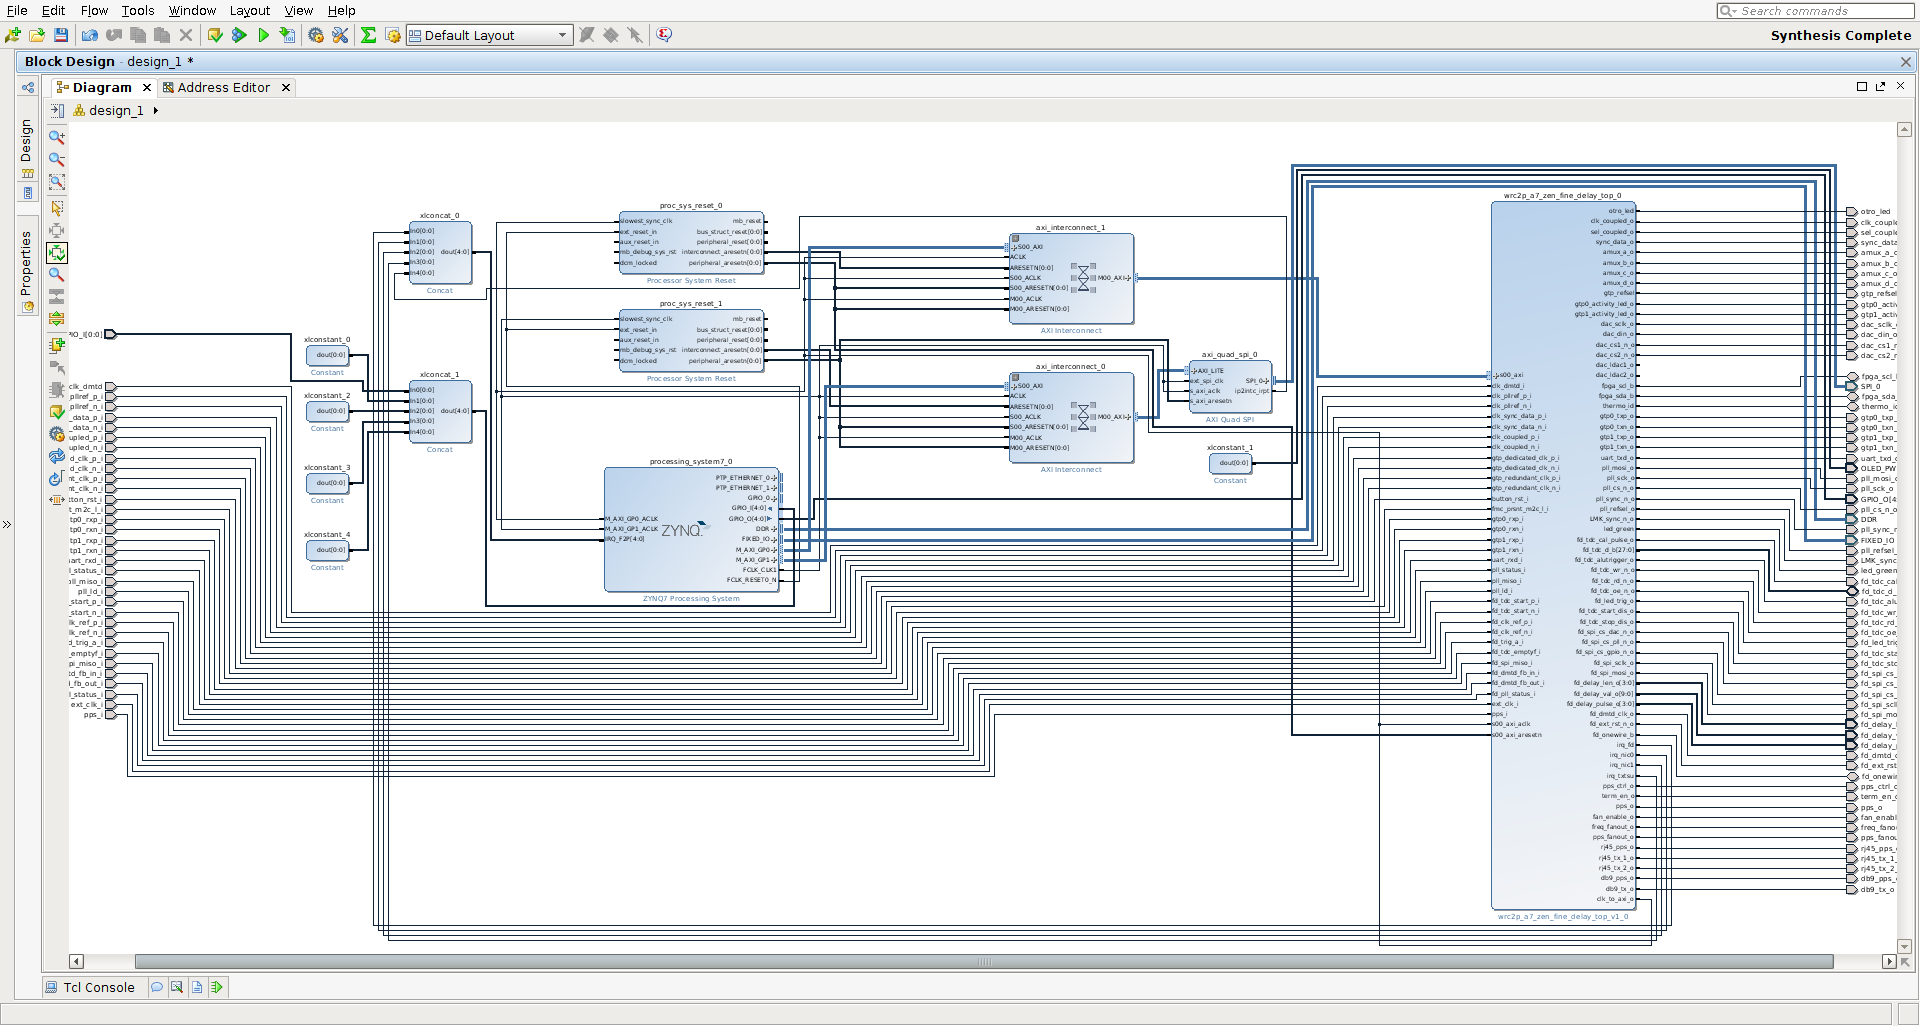
\includegraphics[width=0.8\linewidth]{imagenes/vivado_zen}
	\caption[Captura de Vivado con el diagrama de bloques de la arquitectura 
	del WR-ZEN]{Esta captura muestra el diagrama de bloques generado por Vivado 
	para mostrar los componentes de la arquitectura incluidos en el WR-ZEN.}
	\label{fig:vivadozen}
\end{figure}

El siguiente nivel de abstracción sería a nivel de core-IP donde se encuentra 
el núcleo WR correspondiente a la implementación \gls{wrc2p}. En una primera 
fase de adaptación de la antigua arquitectura de nodo basada en un diseño único 
de \gls{fpga} a la de SoC, se ha mantenido la estructura interna del núcleo WR, 
explicada en la sección ??, realizando cambios únicamente como adaptación a las 
peculiaridades de la familia Zynq-7000. Por ejemplo, se ha necesitado incluir 
un componente que convierta las transacciones del bus Wishbone utilizado en WR 
a las del bus AXI propio de la arquitectura Zynq. En líneas generales el diseño 
HDL \gls{wrc2p} utilizado en el WR-LEN presenta un alto nivel de compatibilidad 
con la nueva plataforma gracias a que la parte PL del modelo Zynq usado es una 
Artix-7. Por ello elementos como los envoltorios de los \textit{transceivers} 
que suele ser algo dependiente de la familia se han podido reutilizar sin 
mayores modificaciones.

\subsection{software}

El gran cambio con respecto al diseño anterior de nodo se encuentra actualmente 
en el ámbito del \textit{sw}. Los diseños anteriores para nodos implementaban 
todo el \textit{sw} de forma embebida, lo que suponía un coste elevado de 
desarrollo debido a la necesidad de un alto conocimiento de la plataforma 
subyacente y del resto de módulos que componen el código del sistema. Gracias a 
la potencia de cálculo extra del núcleo ARM se ha podido incluir un SO tipo 
Linux facilitando en gran medida el desarrollo de nuevas características o la 
inclusión de tecnologías ya existentes en el ecosistema Linux. Para lograr una 
correcta separación entre niveles de abstracción, se ha desarrollado una capa 
de abstracción \textit{hardware} (HAL) así como una serie de drivers que 
permiten acceder a la parte de lógica programable de forma homogénea por el 
\textit{sw} de usuario. Otro aspecto interesante es la mejora en la seguridad 
de los accesos al \textit{hw}, dado que existe una capa intermedia que arbitra 
los accesos evitando accesos indebidos o inconsistencias.

Dado que la complejidad de desarrollo ha aumentado bastante, ha sido necesario 
elaborar una serie de herramientas automáticas para la generación del kernel 
Linux y la compilación del resto de herramientas y \textit{sw} de forma 
parecida al sistema de compilación que existe para el \textit{sw} del 
\gls{wrs}. Dicho sistema automático de compilación se basa en una serie de 
\textit{scripts} que hacen de envoltorio para una herramienta muy conocida en 
este tipo de situaciones (Buildroot) de forma que se evita la necesidad de 
interacción por parte del usuario, facilitando así el despliegue del sistema 
para desarrolladores que necesiten trabajar sobre esta plataforma. El resultado 
es lo que se denomina \textit{root filesystem}, que no es más que una imagen 
del sistema de ficheros Linux para el arranque de la tarjeta.

\incomment{se puede hablar algo más de los módulos existentes (drivers)}

\incomment{esquema de las etapas de arranque}

Sin embargo, dicho \textit{root filesystem} no es lo único que se necesita para 
arrancar la tarjeta. Hay que recordar que se trata de un sistema embebido, por 
lo que se necesita un cargador de arranque inicial que se encargue de las 
tareas más básicas y de bajo nivel como inicializar los componentes \textit{hw} 
de la tarjeta. En la familia Zynq se utiliza un cargador de arranque llamado 
\textit{First Stage Bootloader} (FSBL) que ofrece un conjunto de operaciones 
muy restrigindas dado que no se pretende realizar ninguna tarea de alto nivel 
en esta etapa del arranque. Una de las tareas críticas realizadas por este 
componente de arranque es la inicialización y configuración de la parte PL. La 
última tarea que debe realizar es lanzar un cargador de segunda etapa que ya 
ofrece más flexibilidad a la hora de ser configurado para las necesidades 
específicas de la tarjeta. Además puede ser escogido por el desarrollador, 
contando con dos opciones principalmente que son Barebox y U-boot. Se ha optado 
por el segundo pues ofrece más funcionalidad que el primero y tiene una 
implementación más limpia y actualizada. Esta pieza de \textit{sw} permite 
realizar tareas más complejas de gestión de la tarjeta y termina 
descomprimiendo en memoria el \textit{root filesystem} y lanzando el kernel 
Linux, tras lo cual este toma posesión de la ejecución del procesador.

El desarrollo de todo este sistema ha supuesto un gran esfuerzo por parte de 
mucha gente tanto del grupo de la UGR como de la empresa Seven Solutions. Por 
ello se ha efectuado una primera fase donde se ha preparado el entorno, es 
decir, el SO, los drivers, HAL y demás herramientas de gestión, y se ha dejado 
para otra etapa el aprovechamiento real de la nueva arquitectura desde el punto 
de vista del núcleo de WR.

Por tanto, se mantiene el LM32 en la arquitectura WR. El código del PPSi y el 
resto de \textit{sw} embebido se sigue ejecutando en dicho 
\textit{soft-processor}. Aunque no se haya podido migrar dicho código al ARM, 
se ha conseguido descargar de muchas tareas secundarias de gestión al LM32 que 
si han sido llevadas a nivel de kernel o de usuario. La discusión de la línea 
de trabajo futura y de como organizar el núcleo WR para aprovechar esta nueva 
plataforma SoC se incluye en la sección \ref{sec:socfuturo}.

\section{El nodo WR-ZEN}

Al principio del capítulo ya se introducía una de las características más 
relevantes de esta nueva tarjeta WR llamada WR-ZEN: la incorporación de un SoC 
de la familia Zynq-7000. Gracias a la colaboración con Seven Solutions hemos 
podido disponer en el grupo de la universidad de este nuevo \textit{hw} para 
desarrollar toda la nueva línea de arquitectura y demás producción científica 
asociada a la mejora de WR.

\begin{figure}
	\centering
	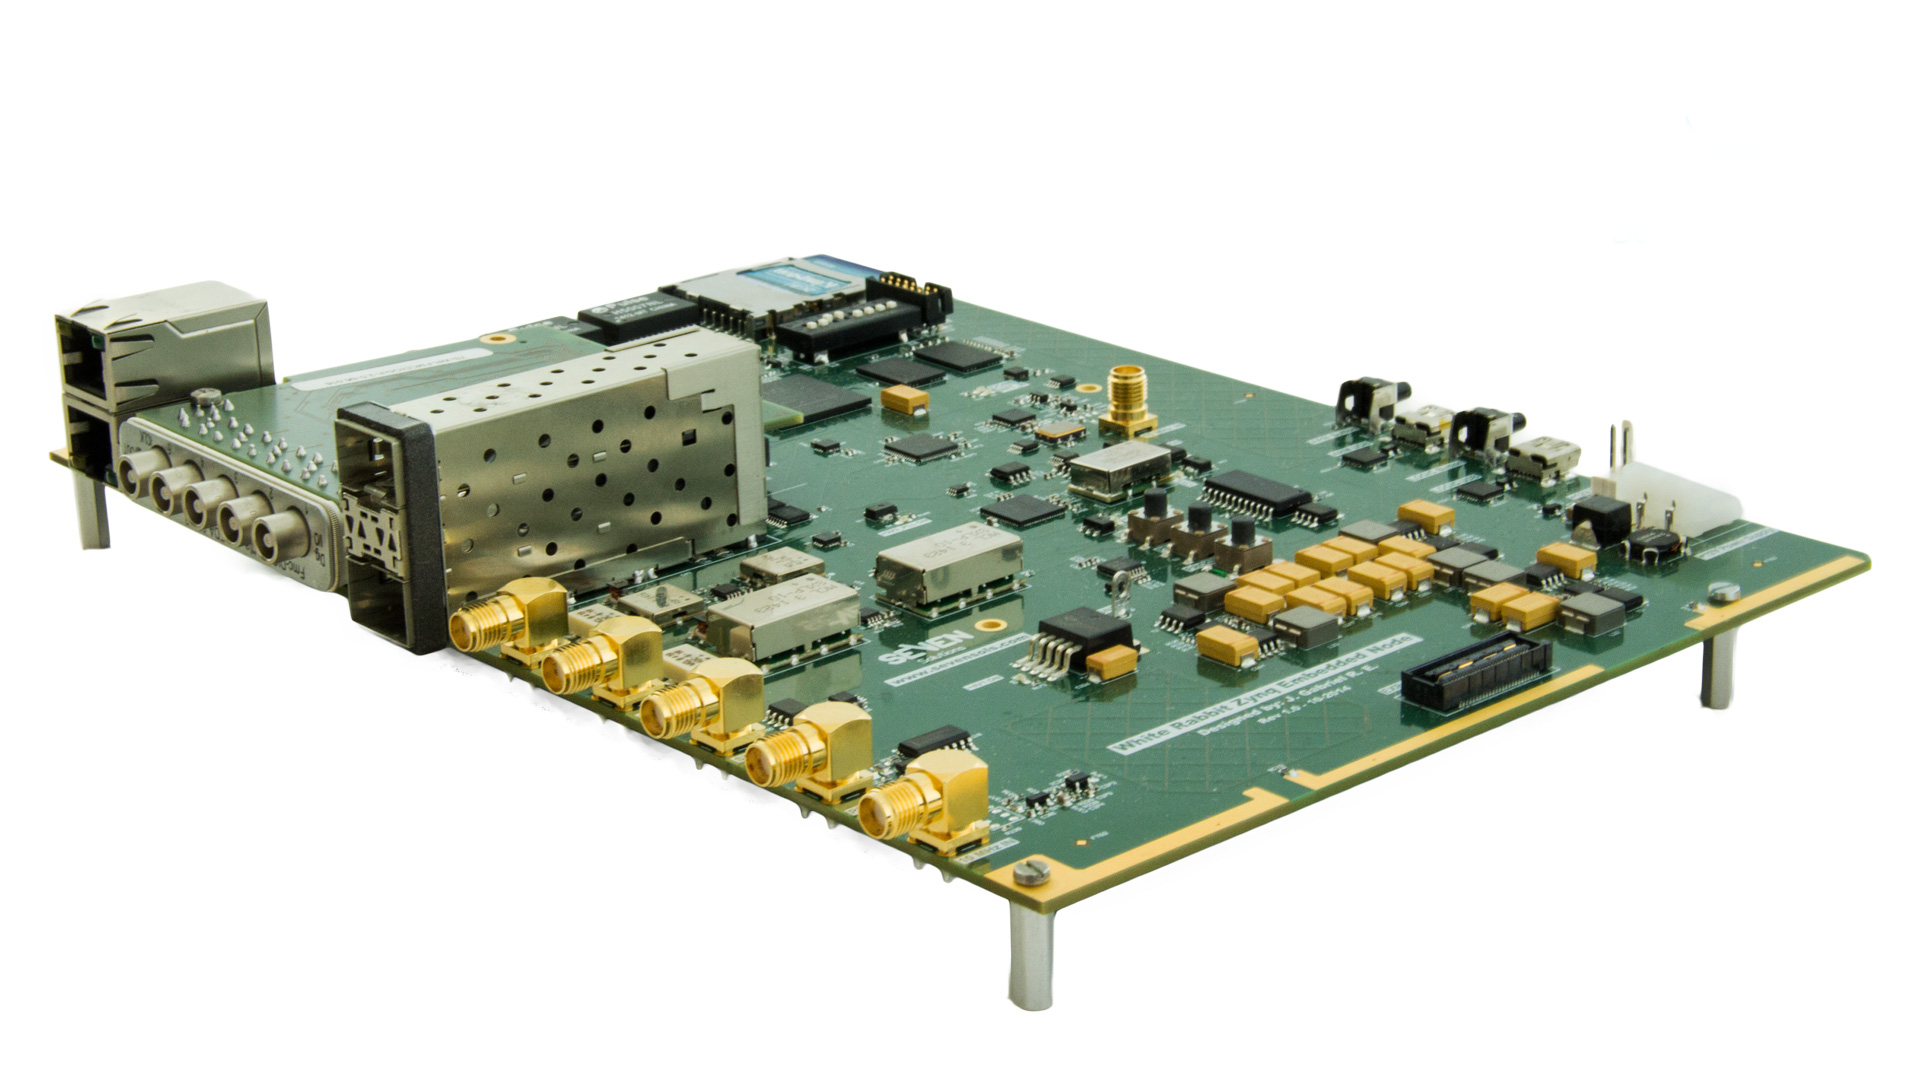
\includegraphics[width=0.7\linewidth]{imagenes/wrzen}
	\caption[Foto de la tarjeta WR-ZEN]{En la imagen de la PCB que forma el 
	nodo WR-ZEN se pueden observar los conectores de e/s SMA, los puertos 
	Ethernet para fibra y cobre, y el conector FMC que tiene una tarjeta de 
	adquisición conectada en la fotografía.}
	\label{fig:wrzen}
\end{figure}

En esta sección se pone el foco en los componentes \textit{hw} incluidos en 
este nuevo nodo ya que se han realizado varios cambios con respecto a la 
electrónica usual incluida en otros dispositivos WR como el \gls{wrs}, 
\gls{spec} o LEN.

\incomment{copiar aquí el párrafo de descripción del hw de la zen}

El nuevo esquema de reloj así como los distintos componentes nuevos que han 
sido introducidos me han permitido profundizar más en la electrónica de 
recuperación y generación de reloj para poder buscar formas de reducir el ruido 
del sistema desde la perspectiva más \textit{hw} del sistema. Dado que esto es 
algo bastante extenso he preferido dedicar un capítulo a parte 
(\ref{cap:reloj}) a todo lo relacionado 
con la electrónica de reloj, explicando como funciona el modelo actual, las 
mejoras al modelo que se investigan para el futuro y algunos resultados de 
pruebas experimentales que suponen una herramienta crucial a la hora de conocer 
este tipo de sistemas.

\section{Conclusiones y Trabajo futuro} \label{sec:socfuturo}

A lo largo de este capítulo se han descrito algunas de las ventajas que ofrece 
migrar la arquitectura del \textit{wrc} (o la variante de doble puerto) para 
nodos WR hacía una nueva plataforma basada en SoC: aumento de las prestaciones 
gracias al soporte \textit{hw} y una mayor flexibilidad de desarrollo gracias a 
la inclusión de un SO tipo Linux. Sin embargo, aún no se ha hecho uso realmente 
de todo el potencial que ofrece la nueva plataforma.

La estructura general presentada en \cite{Daniluk2012} y descrita de forma 
resumida en el diagrama de bloques de la Figura \ref{fig:wrpcinside} muestra 
una arquitectura de bus cuyo nexo de unión entre componentes es el bus Wishbone 
\textit{crossbar}. De esta forma la comunicación entre los diversos módulos y 
el procesador se realiza mediante accesos mapeados a memoria. Esta arquitectura 
deja de tener cierto sentido y se convierte en algo redundante si pensamos en 
la nueva plataforma basada en SoC. Si se realiza una migración de los modulos 
\textit{sw} que actualmente se ejecutan en el LM32, como el PPSi, al procesador 
ARM, es decir, a nivel de SO, ya sea en forma de drivers, o como programas de 
nivel de usuario, resulta que el \textit{sw} de control  necesita pasar primero 
por el puente AXI y luego por el bus Wishbone para llegar a los módulos en la 
parte PL. Por ello se propone una nueva arquitectura que realiza un 
aprovechamiento más eficiente de la nueva estructura de buses del SoC Zynq-7000 
y que se muestra en la Figura ?? \incomment{meter aquí un diagrama con los 
módulos colgando del AXI en vez del wb}. Para ello no habría que reimplementar 
la lógica de los módulos en HDL, si no que sería necesario añadir una capa que 
envuelva o reemplace la lógica de control pensada para el bus Wishbone por la 
del bus AXI. Para facilitar dicha labor se puede desarrollar una herramienta 
similar al \textit{wbgen2} que permita realizar una descripción de los 
registros de un componente en HDL y esta se encarge de generar de forma 
automática toda la lógica de control para la comunicación con el bus.

\incomment{imagen del nuevo esquema con el bus axi}

Sin embargo reemplazar por completo todos los componentes actuales no es algo 
trivial. Hay que tener en cuenta la lógica de control del módulo 
\textit{SoftPLL} que necesita cierto nivel de determinismo en su ejecución para 
realizar el cálculo del desfase y producir los valores consigna que se aplican 
para corregir la frecuencia de oscilación de los cristales disciplinados por WR 
en la tarjeta. Por tanto, se propone una primera fase donde se \textit{suban} 
de nivel el resto de módulos y se mantenga el bus wishbone para la lógica 
encargada del \textit{SoftPLL}. Esto sería una solución intermedia que se 
parece en parte a como funciona el LM32 en la arquitectura tipo \textit{switch}.

Para poder eliminar por completo el bus Wishbone sería necesaria una labor 
previa de investigación que analice y caracterice todo lo relacionado a la 
lógica de control del SoftPLL de manera que se pueda concluir si los requisitos 
temporales que tiene este algoritmo de control se pueden migrar a un sistema 
no-determinista como el Linux que corre ahora mismo a nivel de ARM. Otra 
posibilidad sería implementar la parte \textit{sw} del control del SoftPLL en 
HDL. ¿Por qué no se realizó desde un primer momento? Se podría pensar que es 
algo lógico pues la implementación en \textit{hw} asegura el determinismo y un 
nivel de prestaciones muy superior al alcanzable por la ejecución de un 
algoritmo \textit{sw} en un microprocesador. Sin embargo, hay que tener en 
cuenta que todo el diseño de WR es relativamente nuevo y por tanto, hay 
componentes que debido a su complejidad necesitan de una fase de implementación 
y testeo compleja. Según notas del autor de dicho código \incomment{tomasz 
tenía un documento que decía eso pero no lo encuentro por ningún lado 
ahora...}, esa fue una de las razones por las que parte del algoritmo de 
control se realizan en \textit{sw}. Dado que la tecnología ya cuenta con cierto 
grado de madurez, y que las metodologías de desarrollo para la generación de 
código en HDL han evolucionado mucho en los últimos años, se podría plantear 
una implementación en algún lenguage de descripción hardware de alto nivel como 
System-C, que permita la descripción del algoritmo a un nivel de abstracción 
mayor facilitando el proceso. Esto es algo que actualmente se está investigando 
en el grupo de sincronización de la UGR y que forma parte del núcleo de 
desarrollo de mi futura tésis.

Como conclusión de esta parte destacar la gran oportunidad, desde mi punto de 
vista, que supone el poder disponer de las soluciones en SoC que se están 
desarrollando en los últimos años, como es el caso de la familia Zynq-7000 de 
Xilinx. He podido comprobar de primera mano las restricciones que tiene la 
arquitectura tradicional para nodos basada únicamente en FPGA. Los recursos a 
nivel de \textit{sw} están muy limitados, tanto por el punto de vista del 
colapso del LM32 cuyo objetivo inicial era procesar una única interrupción y 
generar los valores de consigna para los osciladores disciplinados, y al que se 
le han ido añadiendo funcionalidades en forma de \textit{sw} embebido; como por 
la escasez de memoria fruto del uso de FPGAs de perfil bajo. Dado que un 
requisito de este tipo de dispositivos es mantener un coste bajo, no es una 
solución hacer uso de FPGAs con más recursos, lo cual pienso que no sería más 
que un parche pues se seguiría intentado aumentar el número de funcionalidades 
volviendo a colapsar los recursos. Además existe la posibilidad de incorporar 
algún procesador embebido distinto que ofrezca mayor rendimiento, por ejemplo 
el MicroBlaze de Xilinx. De nuevo opino que esto sería un parche y además 
necesitaría de un esfuerzo para adaptar el \textit{sw} a ese procesador. Por 
todo ello, creo que la solución SoC con un procesador físico ARM ofrece el 
mejor compromiso entre prestaciones y coste. Otro punto a su favor es la gran 
aceptación que tiene actualmente este tipo de microprocesadores, haciendo mucho 
más fácil todo lo relativo al desarrollo tanto a nivel de diseño de 
arquitectura como para los programas que se ejecutarán en el mismo.

Queda aún mucho trabajo por hacer para realizar un diseño que aproveche 
realmente las ventajas de la arquitectura ofrecida por la Zynq. Pero es 
importante ver la gran aceptación que está teniendo etre la comunidad 
científica el desarrollo del nodo WR-ZEN, que ya se ha incluido en proyectos de 
gran relevancia internacional como SKA, ya que esto favorece la publicación de 
nuevos artículos científicos que tengan interés en la comunidad relacionados 
con todo la investigación que se está haciendo en torno a este nuevo enfoque 
para nodos WR.

\incomment{ha quedado corto pero tampoco se donde me puedo estirar más}
\chapter{Mejora de la precisión en WR} \label{cap:reloj}

El capítulo anterior ha tratado el sistema desde el punto de vista del 
\textit{firmware}, es decir, la parte en lógica reconfigurable y el 
\textit{software} que se ejecuta en el procesador. Para tener una visión 
completa falta analizar el sistema de relojes encargado de la generación de la 
señal fundamental que mantiene la sincronización en cada dispositivo.

El nuevo diseño basado en SoC-FPGA descrito en el capítulo anterior permite 
incluir una configuración del sistema de reloj flexible que se puede adaptar y 
programar de forma sencilla gracias al nuevo soporte del \textit{Processing 
System} para configurar los elementos \textit{hardware} aún cuando la FPGA no 
ha entrado en funcionamiento. Cambiar la configuración del sistema de reloj era 
posible anteriormente pero requería del soporte de elementos externos ya que si 
se cambia algo relacionado con el reloj de referencia usado por la lógica de la 
FPGA, esta deja de funcionar. 

El algoritmo encargado del cálculo del desfase entre relojes en WR consta de un 
bucle de control, tipo Proporcional Integral (PI), implementado 
en sw y HDL que calcula la 
diferencia en frecuencia y fase del oscilador local con respecto al del nodo 
maestro. Este bucle de control calcula una serie de valores de consigna cuyo 
objetivo es corregir la frecuencia de oscilación del reloj local para ajustarse 
al maestro. Esto se realiza en la electrónica externa a la FPGA en un sistema 
formado por un conversor digital/analógico (DAC), un oscilador controlado por 
tensión (VCXO) y un \gls{pll} que se conectan como muestra la Figura 
\ref{fig:wrclk}.

El nuevo sistema de relojes incluido en el WR-ZEN se muestra en la Figura 
\ref{fig:clknewschema}. En él se pueden observar la inclusión de nuevos 
elementos como un PLL extra en el camino de la referencia principal. Esta 
configuración no está pensada para tener dos PLL en cadena (LMK03806 y 
AD9516-4), si no que se aprovecha una característica del primer PLL para 
distribuir la referencia que le entra a otros componentes sin influir de forma 
negativa en su perfil de ruido. Lo que pretende esta configuración es 
flexibilidad el diseño. Mientras que el LMK03806 tiene unas características de 
ruido muy buenas que permiten disminuir el ruido \textit{suelo}, el PLL 
AD9516-4 ofrece una serie de características que son de bastante utilidad como 
desfases programables para sus salidas. De esta manera se cubren distintos 
tipos de aplicaciones (bajo ruido y las que requieren gran flexibilidad) sin 
necesitar una modificación del PCB. Además se ha registrado la salida de PPS lo 
que consigue que dicha señal presente el perfil de ruido del reloj con el que 
se registra, aumentando así en gran manera su estabilidad frente a la versión 
sin registrar de otros dispositivos WR. Por último se incluye otra mejora 
relevante en el área del módulo para la entrada de una frecuencia externa para 
el modo GM, pero se hará referencia a ello en la sección \ref{sec:gm}.

\begin{figure}
	\centering
	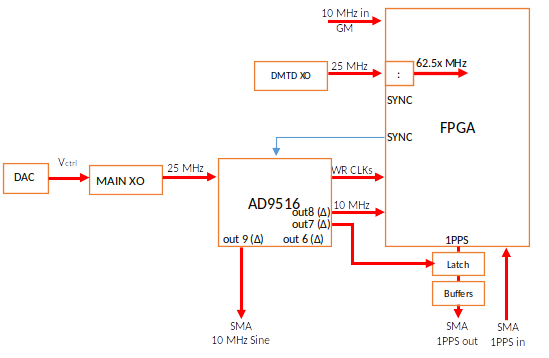
\includegraphics[width=0.7\linewidth]{imagenes/wrclk}
	\caption[Esquema del sistema de reloj en WR]{Esta figura muestra un 
	diagrama de bloques de los componentes principales de la electrónica de 
	relojes para un dispositivo WR.}
	\label{fig:wrclk}
\end{figure}

\section{Caracterización de la nueva plataforma basada en SoC}

El nuevo diseño basado en SoC incluido en el WR-ZEN presenta una serie de 
cambios a nivel de la electrónica de reloj que deben permitir mejorar las 
prestaciones alcanzadas con el resto de dispositivos WR existentes. Dado que 
los cambios en el firmware se encuentran actualmente en desarrollo, y que la 
implementación actual es similar a la presente en el \gls{wrc2p} en el WR-LEN 
la hipótesis de partida es que el rendimiento alcanzado con este nuevo 
dispositivo debe ser almenos equivalente al del WR-LEN. Cumpliendo dicha 
hipótesis se comprueba que la migración a la nueva plataforma no ha supuesto 
ninguna penalización en rendimiento aún cuando la implementación actual no 
aprovecha al máximo todas las ventajas de la nueva plataforma.

Por otro lado se espera que la estabilidad base (es decir sin WR en 
funcionamiento) de la nueva tarjeta sea mayor al resto de equipos actuales como 
el \gls{wrs}, que se usará como modelo de referencia, o el WR-LEN, que también 
será utilizado en las comparativas por incluir la versión de WR basada en el 
\gls{wrc2p}.

Gracias a disponer durante el desarrollo de esta etapa de un medidor de 
\textit{Phase Noise} se ha podido realizar un análisis más exhaustivo que el 
realizado en el capítulo 5. Para caracterizar el nuevo equipo y compararlo con 
los otros dos mencionados anteriormente, se han realizado múltiples medidas de 
ruido de fase para lo cual se ha montado una serie de configuraciones como se 
muestra en la Figura \ref{fig:pnsetup}.




\begin{figure}
	\centering
	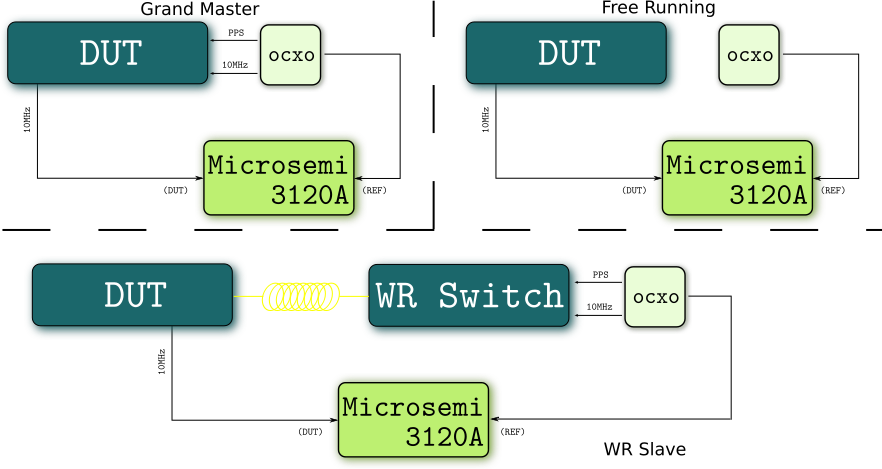
\includegraphics[width=0.7\linewidth]{imagenes/pn_setup}
	\caption[Descripción de la configuración para las pruebas de Phase 
	Noise]{El diagrama muestra las distintas configuraciones utilizadas a la 
	hora de realizar las pruebas para caracterizar el nivel de ruido en los 
	diversos equipos WR. Dependiendo del modo de operación a estudiar se 
	necesita realizar una configuración distinta.}
	\label{fig:pnsetup}
\end{figure}

Para realizar pruebas de ruido de fase se necesita disponer de una referencia 
de reloj lo más estable posible. Esto se debe a que el aparato de medición 
compara dicha señal con la del dispositivo a analizar por lo que cuanto más 
estable sea la señal de referencia, mejores resultados se podrán obtener. En el 
laboratorio se cuenta con un oscilador de tipo OCXO que permite realizar este 
tipo de medidas. En la imagen que acompaña a la Figura \ref{fig:medidapn} se 
puede ver por qué es tan estable este tipo de osciladores: presenta una gran 
capa aislante además de controles que compensan el cambio de temperatura para 
mantener lo más estable posible la frecuencia. A su lado también se puede ver 
un GPSDO que se utiliza en algunas ocasiones como referencia en para este tipo 
de pruebas.

\begin{figure}
	\centering
	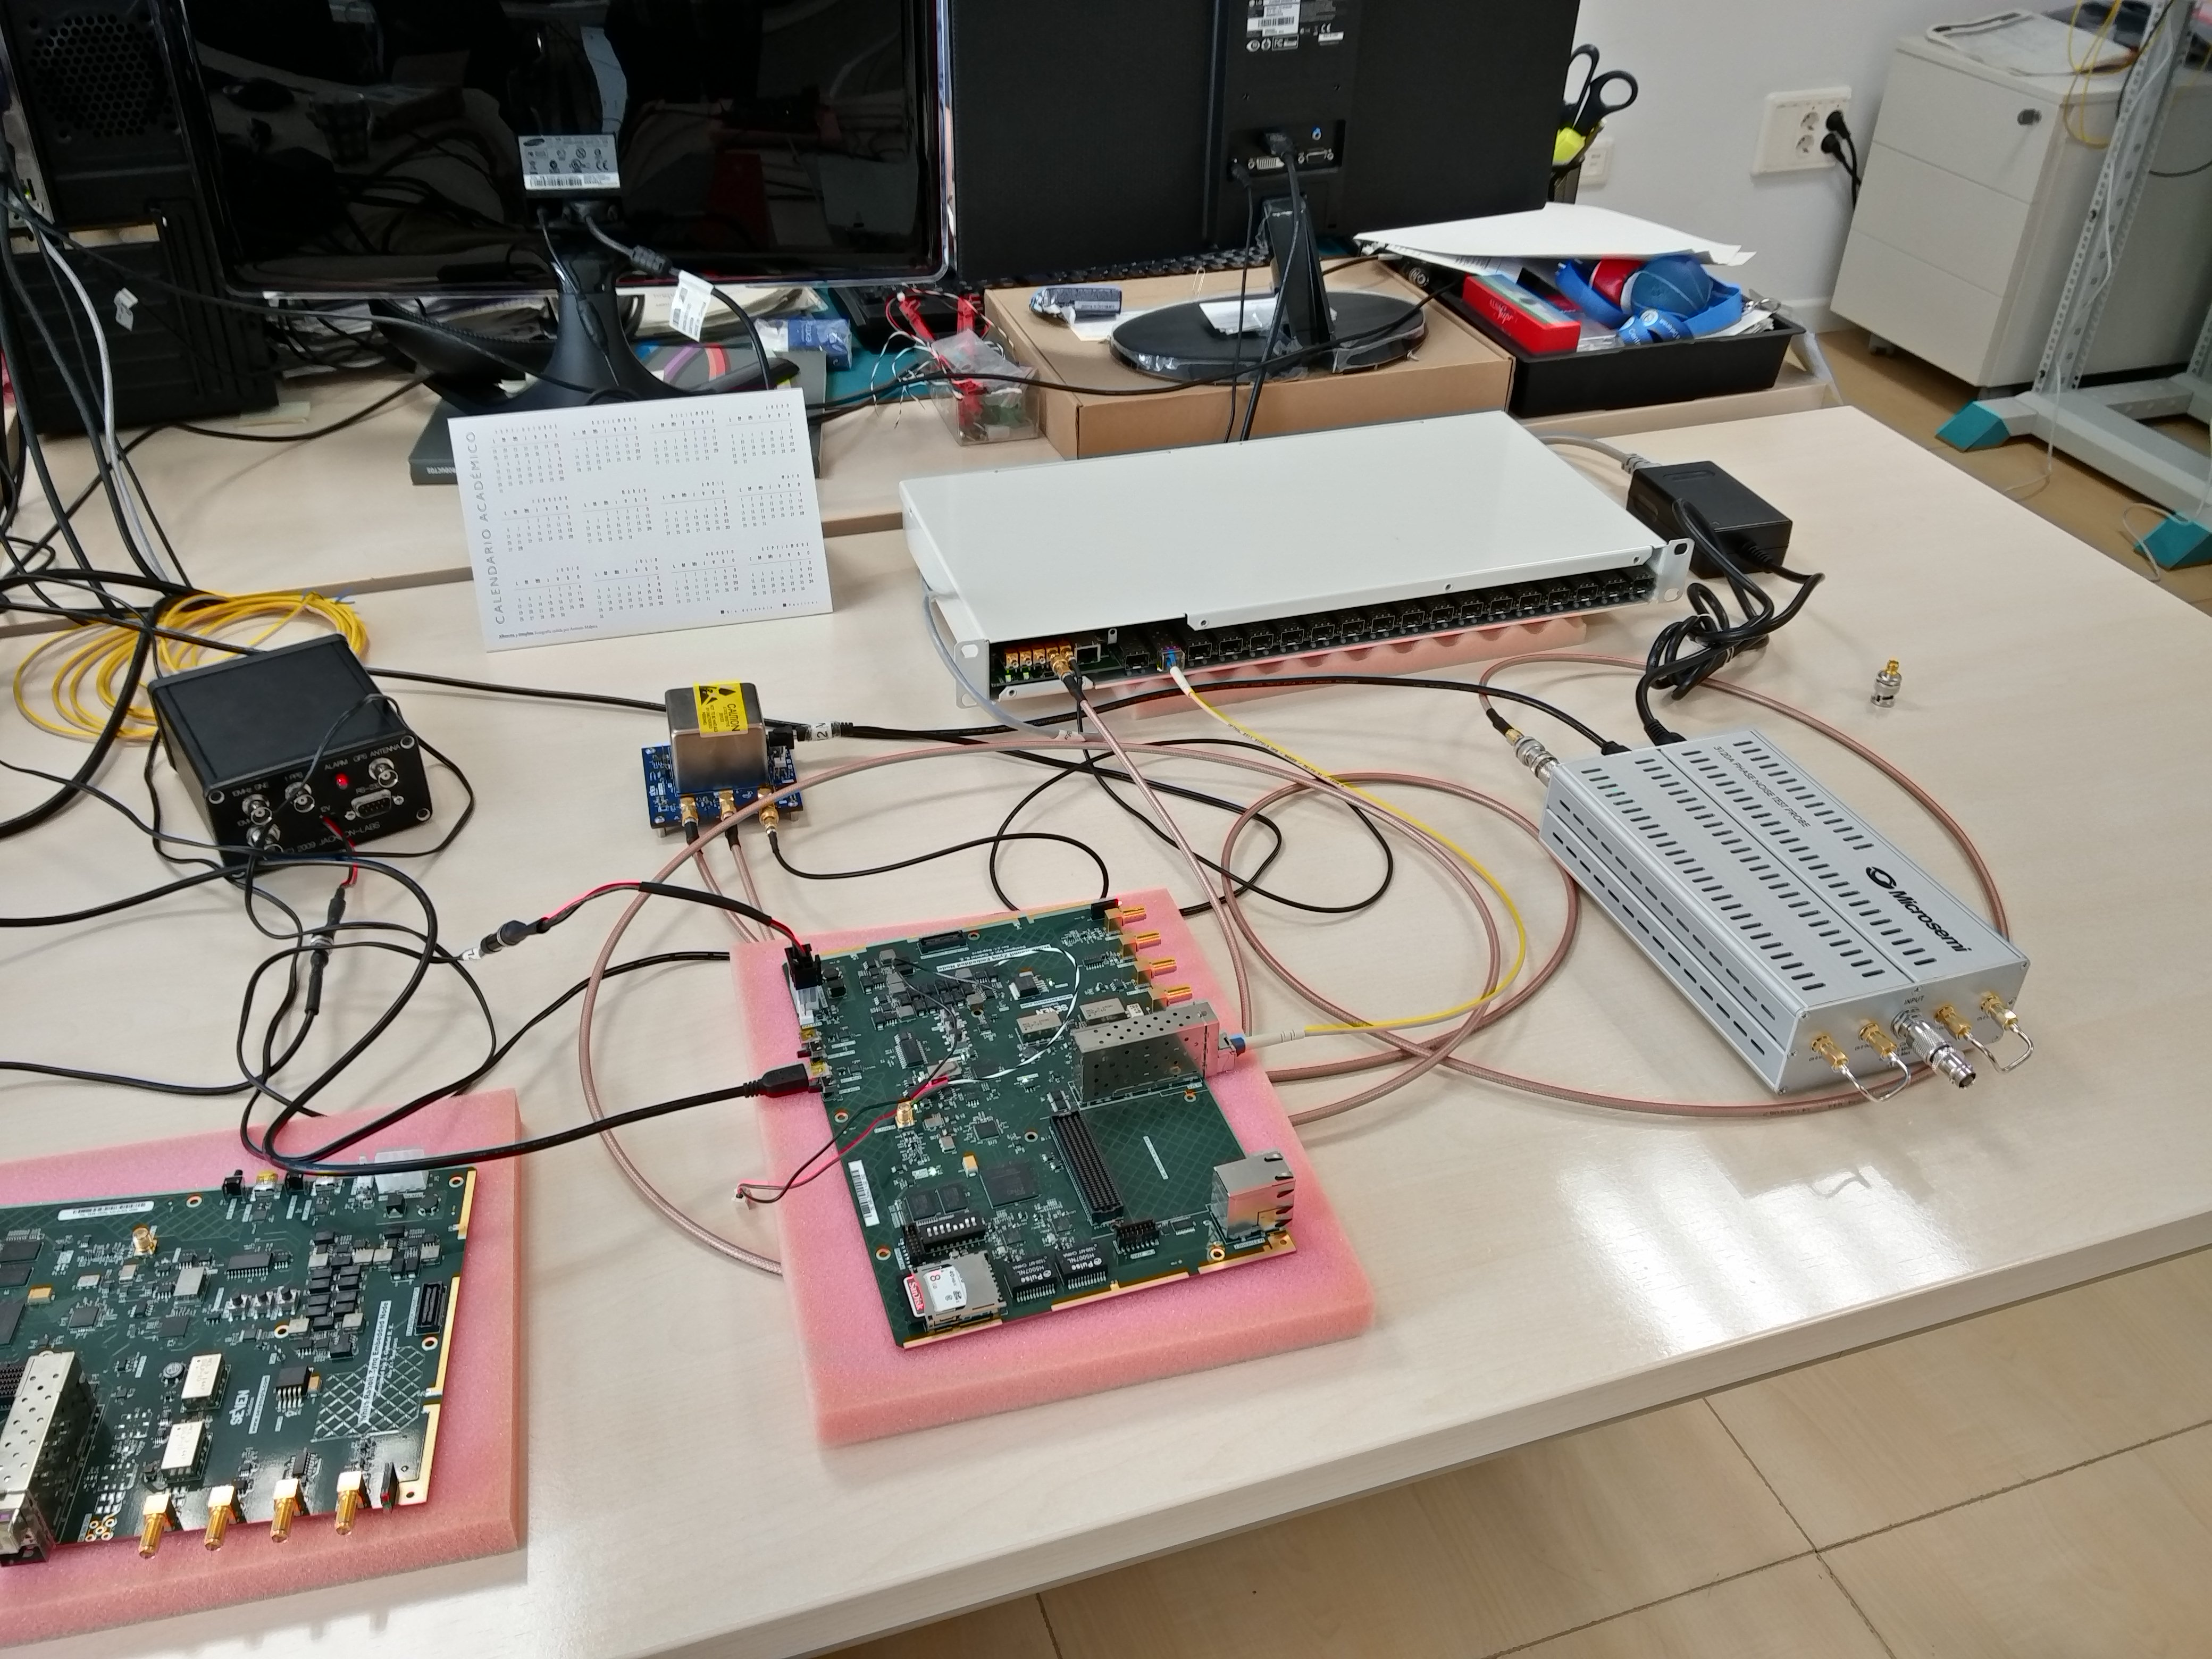
\includegraphics[width=0.7\linewidth]{imagenes/medida_pn}
	\caption[Imagen de la toma de medidas de \textit{Phase Noise}]{La imagen 
	muestra los equipos utilizados para realizar las pruebas de ruido.}
	\label{fig:medidapn}
\end{figure}

Los primeros resultados obtenidos caracterizan el ruido de fase para la 
frecuencia de salida de 10 MHz, generada a partir de la frecuencia de 
referencia disciplinada por WR, para el WR-ZEN. 

\begin{figure}
	\centering
	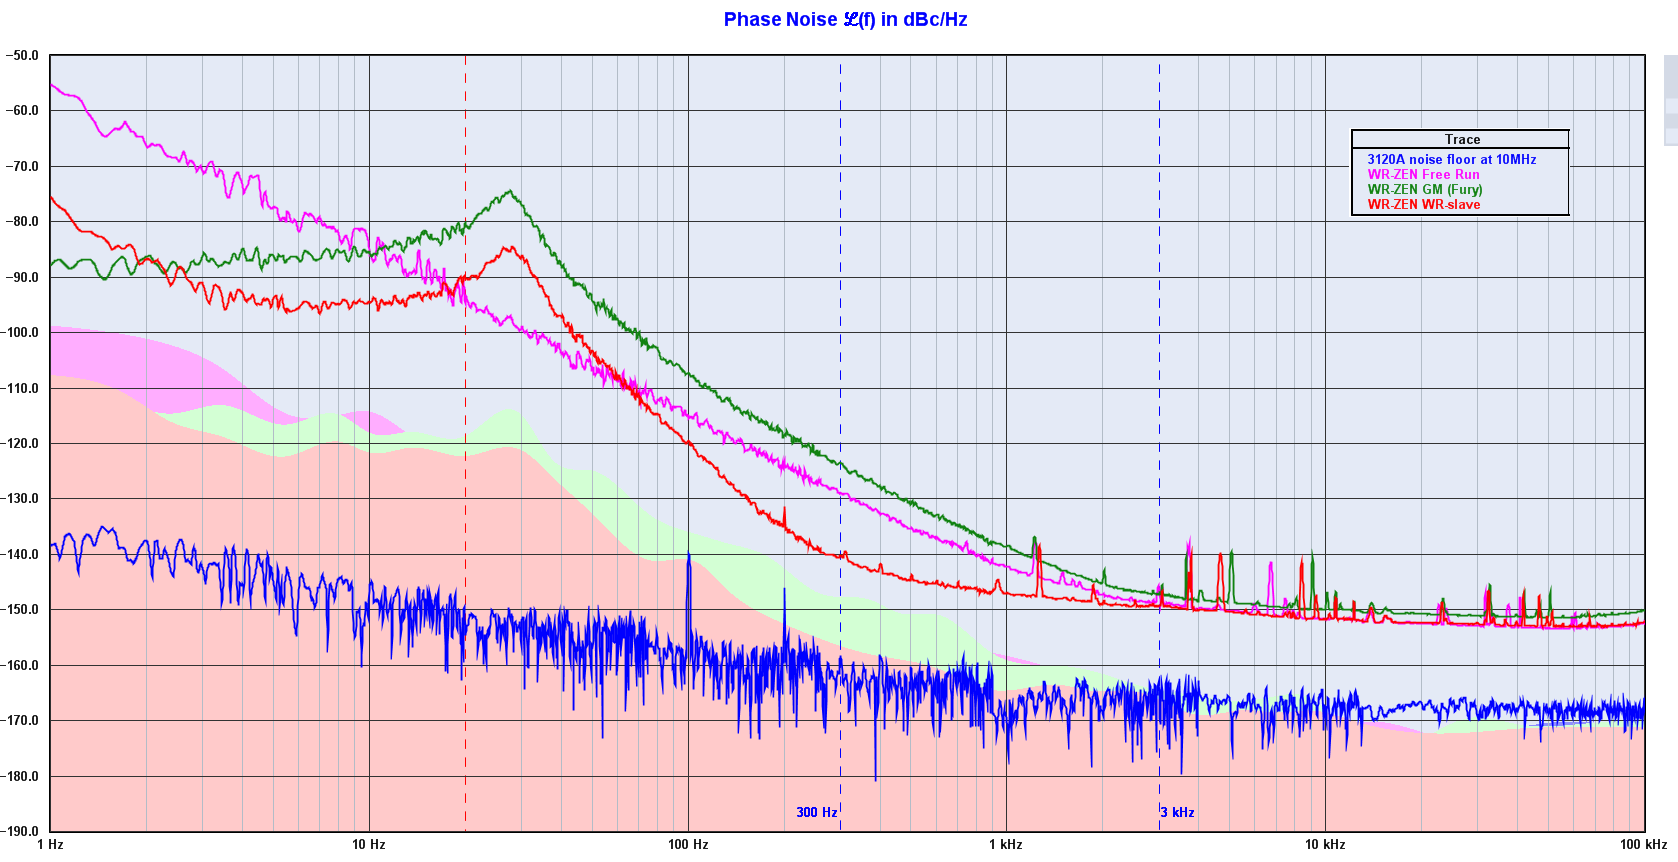
\includegraphics[width=\linewidth]{imagenes/wrzenpn}
	\caption[Gráfico de ruido de fase para el WR-ZEN]{En este gráfico se 
	incluyen los resultados de las medidas de ruido de fase para caracterizar 
	el nivel de ruido presente en el equipo WR-ZEN en los tres modos de 
	operación posibles: maestro \textit{free-running}, maestro GM y nodo 
	esclavo.}
	\label{fig:wrzenpn}
\end{figure}

De forma resumida se comentan los aspectos clave de la información que se puede 
extraer de este tipo de medidas. La línea azul corresponde al ruido base que 
tiene el aparato, es decir, usando el 3120A no se puede medir señales que 
presenten un nivel de ruido inferior al delimitado por la línea azul. Para 
obtenerlo se utiliza el reloj de referencia y mediante el uso de un conector en 
T se divide la señal para usarla como referencia y como señal para el 
dispositivo a medir (\textit{Device Under Test}, DUT). La línea rosa 
corresponde al modo maestro \textit{free running} (la referencia global es su 
propio oscilador local). Las líneas verde y roja corresponden a los modos GM y 
esclavo respectivamente. Se observa el diagrama de Bode típico de un filtro 
paso-bajo. El bucle de control de WR actúa como un filtro que responde ante 
cambios de baja frecuencia sobre la referencia y elimina los producidos en alta 
frecuencia. La frecuencia de corte del filtro se sitúa en torno a los 30 Hz 
como se puede ver en el gráfico. El perfil de ruido final (suelo) que muestra 
el diagrama en \textit{offsets} de alta frecuencia viene limitado por las 
características del PLL utilizado para generar las frecuencias usadas en WR a 
partir del XO de referencia.

\begin{figure}
	\centering
	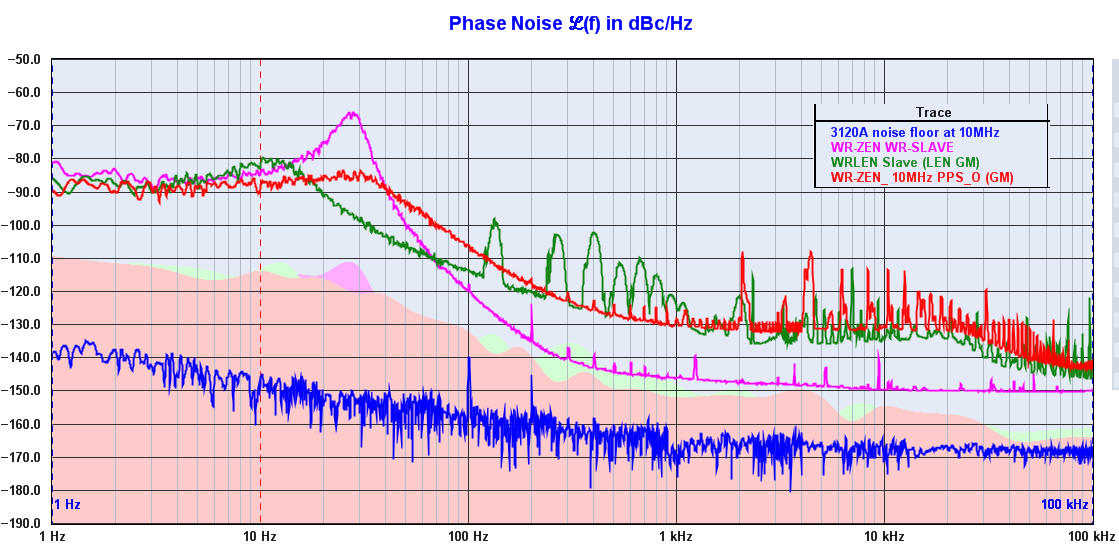
\includegraphics[width=\linewidth]{imagenes/zen_len_comp}
	\caption[Comparativa de \textit{Phase Noise} entre WR-ZEN y WR-LEN]{Este 
		gráfico acompaña una comparativa para los modos esclavo entre el WR-ZEN 
		y 
		el WR-LEN. Además se incluye (línea roja) el resultado de algunas 
		mejoras 
		en el WR-ZEN.}
	\label{fig:zenlencomp}
\end{figure}

\section{Comparativa con otros equipos WR}

Para verificar que la migración a la plataforma Zynq del \gls{wrc2p} y los 
cambios realizados en la electrónica del sistema de reloj no presentan 
problemas se han realizado una serie de medidas de forma similar a las ya 
realizadas para el WR-ZEN (versión de \textit{hw} 2) de manera que se pueda 
comprobar las hipótesis 
planteadas al principio y comprobar que el nuevo desarrollo funciona 
correctamente.

El \gls{wrs} se ha utilizado ya que representa el dispositivo de referencia en 
el mundo \gls{wr}. Las medidas de ruido de fase se han tomado siguiendo la 
misma configuración mostrada en la Figura \ref{fig:pnsetup}. Los resultados se 
acompañan en la Figura \ref{fig:compall}. Para calcular el \textit{jitter} en 
unidades de tiempo se integra el área correspondiente a cada gráfica con 
límites en 1 Hz y 100 kHz, los valores obtenidos se encuentran en la Tabla 
\ref{fig:compall}. 

\begin{figure}
	\centering
	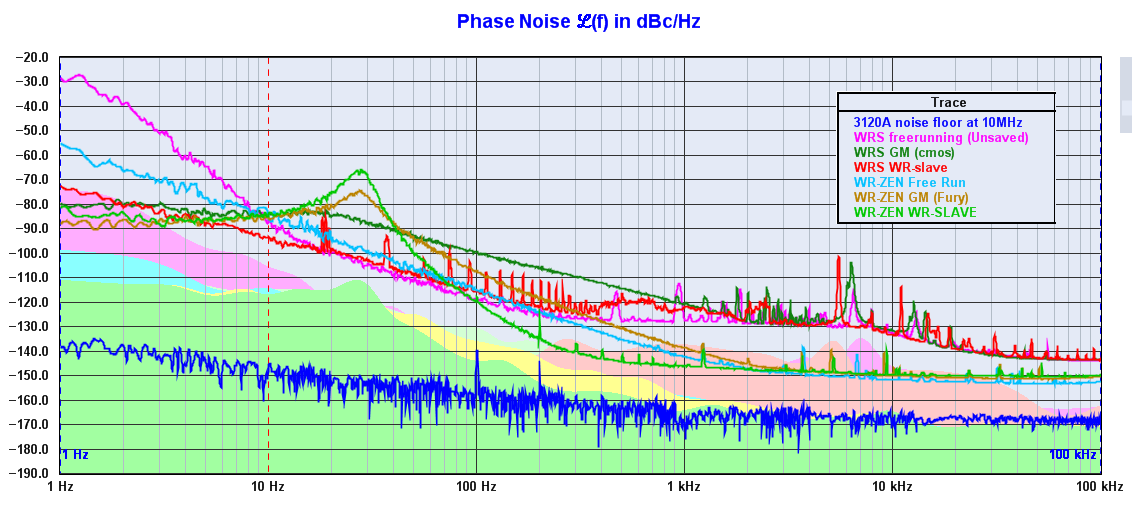
\includegraphics[width=\linewidth]{imagenes/comp_all}
	\caption[Comparativa de \textit{Phase Noise} entre WRS y WR-ZEN]{En este 
	gráfico se muestra la comparativa de ruido de fase entre WRS y WR-ZEN en 
	los tres modos de funcionamiento: maestro \textit{free-running}, maestro GM 
	y esclavo.}
	\label{fig:compall}
\end{figure}

Los resultados muestran que aún queda trabajo por hacer para conseguir el 
objetivo de mejorar las prestaciones para el nodo WR-ZEN. Si se observa los 
perfiles de ruido correspondientes a el modo \textit{free running} se constata 
una gran mejora en la estabilidad gracias a la incorporación de un oscilador 
mucho más estable en el WR-ZEN. Sin embargo, para el resto de gráficas se 
observa una mejor estabilidad en el WRS.

\begin{table}
	% increase table row spacing, adjust to taste
	\renewcommand{\arraystretch}{1.3}
	% if using array.sty, it might be a good idea to tweak the value of
	% \extrarowheight as needed to properly center the text within the cells
	\caption{Valores RMS \textit{jitter} para los resultados de la Figura 
	\ref{fig:compall}.}
	\label{tab:compall}
	\centering
	% Some packages, such as MDW tools, offer better commands for making tables
	% than the plain LaTeX2e tabular which is used here.
	\begin{tabular}{|c||c|}
		\hline
		Dispositivo (modo) & RMS Jitter 1Hz-100kHz (ps) \\
		\hline
		WR-ZEN maestro \textit{free-running} & 25 \\
		\hline
		WRS maestro \textit{free-running} & 620 \\
		\hline
		WR-ZEN maestro GM & 14 \\
		\hline
		WRS maestro GM & 9.4 \\
		\hline
		WR-ZEN esclavo & 30 \\
		\hline
		WRS eclavo & 5.6 \\
		\hline
	\end{tabular}
\end{table}

Para determinar que está limitando mejorar el rendimiento obtenidos por el WRS 
se ha realizado una labor de análisis de los distintos componentes que 
intervienen en el sistema de sincronización. Las conclusiones a las que se ha 
llegado han sido que se necesita optimizar los parámetros del bucle de control 
PI en el WR-ZEN además de adaptar ciertos elementos en la circuitería relativa 
al sistema de reloj. Todo ello viene motivado por los cambios que se han 
realizado en el \textit{hw} con respecto al sistema de referencia utilizado en 
WR.

La Figura \ref{fig:zenlencomp} muestra una pequeña comparativa entre dos nodos 
que incluyen la implementación \gls{wrc2p} en modo esclavo. Según la hipótesis 
de partida, el resultado para ambos debería ser equivalente pues el algoritmo 
de control ha sido migrado sin realizar más cambios que los necesarios para 
ajustarse a la nueva plataforma Zynq. Como en el caso anterior de la 
comparativa con el WRS, el WR-ZEN presenta un rendimiento inferior. Tras la 
labor de análisis se determinó que el \textit{overshoot} visto en torno 20 Hz 
se debía a un cálculo incorrecto en un filtro RC que se encuentra a la salida 
del oscilador principal. Tras modificar el circuito de manera experimental en 
el laboratorio se consiguió reducir dicho fenómeno obteniendo los resultados 
correspondientes a la línea roja de la Figura \ref{fig:zenlencomp}.

\begin{figure}
	\centering
	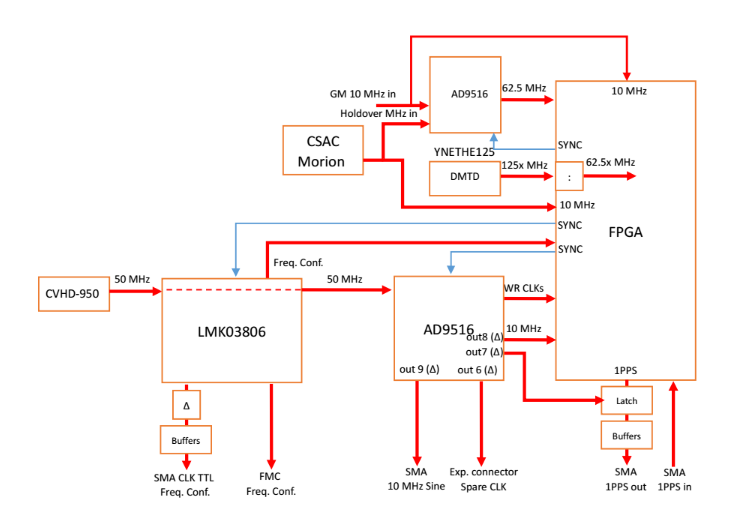
\includegraphics[width=\linewidth]{imagenes/clknewschema}
	\caption[Nuevo esquema de reloj incluido en el WR-ZEN v3.0]{El nuevo 
		esquema de reloj incluido en el WR-ZEN v3.0 incluye las mejoras 
		desarrolladas en el CERN para el modo GM con el PLL externo. Además se 
		pueden apreciar otros cambios con respecto a la electrónica de reloj 
		tradicional.}
	\label{fig:clknewschema}
\end{figure}

Inicialmente había una diferencia en RMS \textit{jitter} entre ambos equipos de 
22.3 ps, y tras el cambio del filtro RC se ha conseguido bajar a 0.8 ps lo que 
equipara prácticamente a ambos dispositivos en rendimiento. Sin embargo, 
gracias a las mejoras realizadas en el \textit{hw} del WR-ZEN el valor de 
\textit{jitter} debería ser menor si se compara con el WR-LEN. En la figura se 
aprecia como el ancho de banda del bucle PI en el caso del WR-ZEN es mayor, 
influyendo en el valor final de RMS \textit{jitter}. La zona fuera del bucle de 
control (alta frecuencia) es mucho más limpia como cabía esperar y no presenta 
el nivel de ruido que si se observa en el caso del WR-LEN.

\section{Línea actual de mejora} \label{sec:gm}


La línea de investigación que se sigue actualmente se centra en mejorar los 
elementos cuyo nivel de ruido limitan la mejora global del sistema. Uno de los 
aspectos clave es el rendimiento alcanzable por el modo \acrlong{gm}. Si 
recordamos en los capítulos iniciales se hace referencia al interés por usar WR 
en centros de metrología (entre otros) para poder distribuir sus costosas y muy 
estables referencias de tiempo a otras instituciones. Sin embargo, actualmente 
el nivel de ruido presente en la electrónica de control utilizada para el modo 
GM presenta una limitación importante en cuanto a rendimiento. Por tanto, no 
sirve de nada tener una referencia muy buena si el sistema utilizado para 
distribuirla la empeora demasiado. 

Este movimiento está liderado por el CERN \cite{mattia2016-2} que ha realizado 
una serie de modificaciones en la electrónica del WRS para incorporar un nuevo 
sistema de PLL que enlaza la frecuencia externa sin necesidad del sistema usado 
hasta ahora en lógica reconfigurable. En resumen, se prescinde de los elementos 
PLL y de generación de señales de reloj internos de la FPGA en favor de 
componentes externos que ofrecen perfiles mucho más bajos de ruido. Este 
movimiento resta flexibilidad y aumenta el coste a cambio de aumentar 
notablemente el rendimiento del sistema.

\begin{figure}[H]
	\centering
	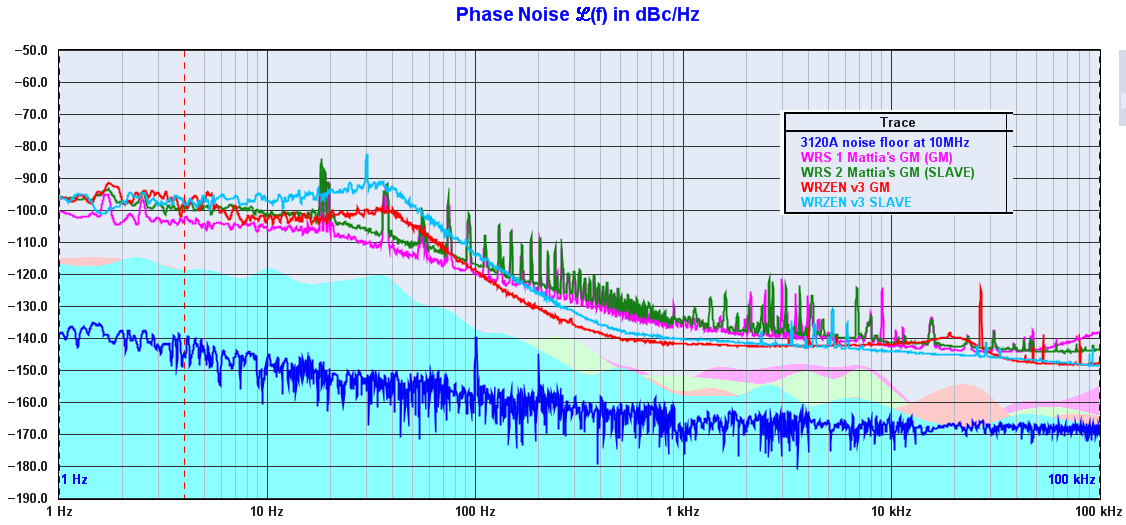
\includegraphics[width=\linewidth]{imagenes/gm_mattia}
	\caption[Resultados de la mejora del modo GM]{Esta gráfica muestra la 
		mejora en el rendimiento obtenido en el WRS y el WR-ZEN gracias a la 
		mejora 
		del modo GM con la incorporación de hw externo a la FPGA para enlazar a 
		la 
		fuente de reloj externa.}
	\label{fig:gmmattia}
\end{figure}

Basándose en el trabajo de Mattia Rizzi en el Cern se han introducido mejoras 
en el diseño del WR-ZEN (de la futura versión de \textit{hw} 3) siguiendo la 
misma línea de incorporar soporte 
\textit{hw} específico para el modo GM. Los resultados se pueden comprobar en 
la Figura \ref{fig:gmmattia} y la Tabla \ref{tab:gmmattia}. Como se puede 
comprobar la mejora ha sido muy relevante, llegando a valores cercanos a 
reducir la barrera del ps. Al igual que en los resultados previos se observa un 
mayor nivel de ruido en el WR-ZEN en comparación con el WRS. Actualmente se 
está realizando una labor de optimización del bucle de control PI en el WR-ZEN 
para conseguir reducir el ancho de banda del bucle y lograr reducir la barrera 
del ps.

\begin{table}
	% increase table row spacing, adjust to taste
	\renewcommand{\arraystretch}{1.3}
	% if using array.sty, it might be a good idea to tweak the value of
	% \extrarowheight as needed to properly center the text within the cells
	\caption{Valores RMS \textit{jitter} para la modificación del modo GM en el 
		WRS y el WR-ZEN.}
	\label{tab:gmmattia}
	\centering
	% Some packages, such as MDW tools, offer better commands for making tables
	% than the plain LaTeX2e tabular which is used here.
	\begin{tabular}{|c||c|}
		\hline
		Dispositivo (modo) & RMS Jitter 1Hz-100kHz (ps) \\
		\hline
		WR-ZEN GM mejorado & 1.7 \\
		\hline
		WRS GM mejorado  & 1.5 \\
		\hline
		WR-ZEN esclavo mejorado & 3.4 \\
		\hline
		WRS esclavo mejorado & 2.0 \\
		\hline
	\end{tabular}
\end{table}

\section{Conclusiones}

Toda la circuitería encargada del sistema de generación y recuperación de la 
referencia de reloj utilizada en WR es un sistema clave si se pretende lograr 
una mejora en el rendimiento alcanzado por este protocolo. Los cambios vistos 
en anteriores capítulos pueden mejorar la flexibilidad del diseño gracias al 
uso de nuevas plataformas basadas en SoC y también pueden lograr cierto nivel 
de mejora en las prestaciones aunque en este apartado la mayor parte del ruido 
del sistema se debe a la circuitería utilizada para el sistema de relojes.

Por ello no basta con realizar cambios en el \textit{firmware} si no que es 
necesario emprender una labor de caracterización y análisis de los componentes 
que intervienen en dicha circuitería. Dada mi formación como informático mi 
contribución a este aspecto se ve más limitada por mi conocimiento de 
electrónica. Sin embargo puedo aportar mi granito de arena colaborando en 
realizar análisis que permitan detectar posibles mejoras que luego serán 
realizadas por los diseñadores de circuitos electrónicos. También es clave la 
caracterización de los equipos ya que permite determinar el rendimiento real 
del sistema comprobando si se han cumplido las hipótesis de diseño iniciales.

Con el diseño del WR-ZEN se buscaba mejorar el rendimiento global para la 
arquitectura de nodo basada en el \textit{wrc2p}, motivo de ello es la 
incorporación de nuevos componentes que sobre el papel ofrecen mejores 
características que los utilizados en los diseños de referencia de WR. Además 
la nueva arquitectura basada en SoC ha permitido realizar un diseño flexible 
que es capaz de adaptar múltiples configuraciones del sistema de reloj para 
conseguir un menor ruido, \textit{offsets} programables, etc. Esta nueva 
configuración es de gran ayuda durante la labor de investigación pues permite 
probar múltiples configuraciones distintas sin necesitar cambios a nivel de 
rediseño de la PCB. 

Sin 
embargo, los resultados obtenidos, aunque son buenos, evidencian el hecho de 
que todavía queda trabajo por hacer. Se ha comprobado que la nueva circuitería 
de reloj ofrece un perfil de ruido más bajo y limpio que en modelos anteriores, 
pero el rendimiento obtenido está todavía por debajo de las expectativas.

Actualmente estoy trabajando en seguir mejorando el rendimiento en el WR-ZEN 
enfocándome en el bucle de control PI para jugar con el ancho de banda del 
mismo para intentar reducir el ruido observado en los resultados anteriores.

\section{Aplicaciones}

Los nodos WR eran típicamente dispositivos muy simples que estaban pensados 
para su uso como parte de un sistema mayor. Ejemplo de ello es la tarjeta SPEC, 
pensada para ser conectada a un puerto PCIe de un PC. Aunque existen nodos como 
el WR-LEN que pueden actuar perfectamente de forma autónoma, a la hora de 
integrar el nodo WR dentro de una aplicación mayor surgen varias deficiencias 
que se han tratado de solventar con la inclusión de la arquitectura basada en 
SoC-FPGA. Sobre todo cabe destacar el alto coste de desarrollo que tiene añadir 
cualquier funcionalidad a la arquitectura de nodo inicial y la falta de 
recursos para hacerlo. Gracias al nuevo diseño muchas más aplicaciones pueden 
adaptar a sus necesidades el diseño actual ya que incluir nuevos protocolos o 
aplicaciones de usuario es relativamente sencillo gracias al soporte de drivers 
y de la capa de abstracción hardware que permiten abstraer a los 
desarrolladores de la implementación de más bajo nivel del sistema.
Así mismo las mejoras realizadas en el ámbito de las prestaciones posibilitan 
la utilización de la tecnología WR en aplicaciones con altos requisitos de 
sincronización, como nuevas instalaciones científicas (SKA por ejemplo) o la 
distribución de frecuencia con limitación al ruido del sistema. La reducción 
del \textit{jitter} del sistema es algo que se está demandando desde el sector 
metrólogico. Estas instituciones necesitan propagar su referencia de tiempo con 
la mínima degradación posible, así que cualquier mejora en este sentido será 
recibida con los brazos abiertos por dicho sector. Por otra parte otro campo 
que se verá beneficiado es el distribución de tiempo con enlaces de muy larga 
distancia, donde también es clave mantener un perfil de ruido bajo para 
compensar el deterioro provocado por la longitud del enlace.

Parte de los resultados obtenidos en este trabajo también se enfocan en la 
escalabilidad y los limites de la tecnología con el foco en aplicaciones menos 
exigentes. Los experimentos han permitido determinar el número máximo de nodos 
que actualmente soporta la implementación basada en \gls{wrc2p} en el WR-LEN, 
cuyos resultados son extrapolables a otros equipos WR gracias al mantenimiento 
de la electrónica de referencia en el dispositivo utilizado para dichas 
pruebas, y además los valores de exactitud en la sincronización en cadenas 
largas de dispositivos. Estos datos son de gran importancia a la hora de elegir 
esta tecnología en aplicaciones con redes con muchos nodos conectados en 
cadena, telecomunicaciones o grandes factorías son ejemplos. 


\chapter{Conclusión y trabajo futuro}

\backmatter
\nocite{*}
\addcontentsline{toc}{chapter}{Bibliografía}
\bibliographystyle{plain}
\bibliography{bibliografia/wr_bib}


\appendix
%\input{apendices/manual_usuario/manual_usuario}
%%\input{apendices/paper/paper}
%\input{glosario/entradas_glosario}
\addcontentsline{toc}{chapter}{Lista de Acrónimos}
\printglossaries

\thispagestyle{empty}

\end{document}
